\documentclass[12pt]{article}
\usepackage[letterpaper, left=0.6in, right=0.6in, top=0.95in, bottom=0.95in,
  headheight=15pt, headsep=0.25in, footskip=0.45in]{geometry}
\usepackage[T1]{fontenc}
\usepackage[default]{sourcesanspro}
\usepackage{inconsolata}
\usepackage{textcomp}
\usepackage{microtype}
\usepackage{tikz}
\usetikzlibrary{arrows.meta}
\usepackage{fancyhdr}
\pagestyle{fancy}
\fancyhf{}
\fancyhead[L]{Week 4 / Stars and wheels / K--1}
\fancyfoot[L]{Bellingham Math Circle / Week 4 / F04-K-v4}
\fancyfoot[R]{\thepage}
\renewcommand{\headrulewidth}{0pt}
\setlength{\parindent}{0pt}
\setlength{\parskip}{0pt}
\newcommand{\prob}[1]{\textbf{Problem #1:}}
\newcommand{\bx}{\hspace{0.07in}\begingroup\setlength{\fboxsep}{0pt}\setlength{\fboxrule}{0.8pt}\raisebox{-0.11in}{\framebox[0.42in]{\rule{0pt}{0.34in}}}\endgroup}
\newcommand{\blank}{\rule[-3pt]{0.85in}{0.6pt}}
\pagenumbering{arabic}
\begin{document}
\fontsize{14}{19}\selectfont
\par\vspace{0in}\noindent To hop 2, move the counter 2 dots along the way the arrow points.\par
\vspace{0.14in}
\par\vspace{0in}\noindent \prob{1} Put a counter on the black dot and hop it until it is back. Draw each hop on a small ring, and circle each hop that lands on every dot.\par
\par\vspace{0.15in}\noindent\makebox[\textwidth][c]{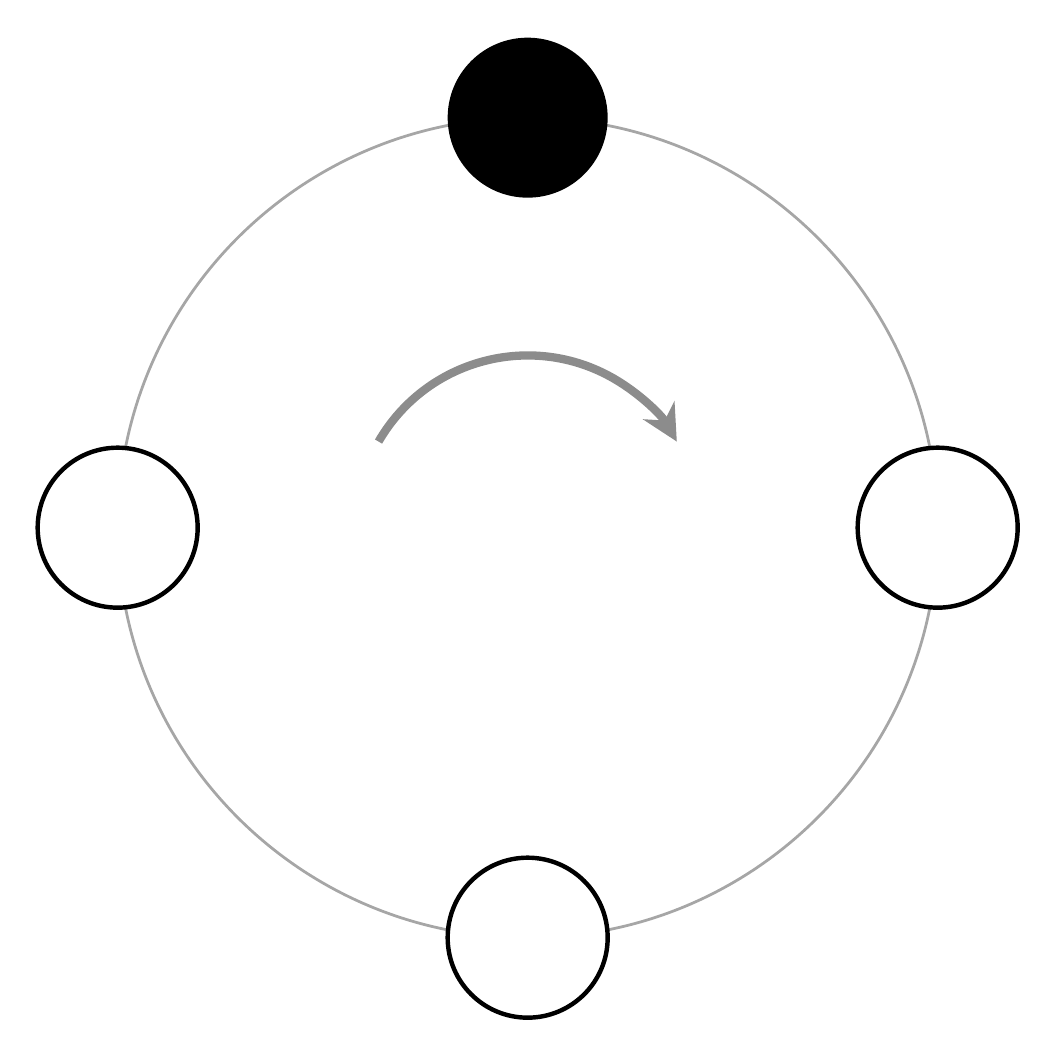
\begin{tikzpicture}[x=1in,y=1in]
\useasboundingbox (-2.5,-2.5) rectangle (2.5,2.5);
\draw[black!35, line width=1pt] (0,0) circle (2.05);
\fill[black] (0,2.05) circle (0.4);
\filldraw[fill=white, draw=black, line width=1.6pt] (2.05,0) circle (0.4);
\filldraw[fill=white, draw=black, line width=1.6pt] (0,-2.05) circle (0.4);
\filldraw[fill=white, draw=black, line width=1.6pt] (-2.05,0) circle (0.4);
\draw[black!45, line width=3pt, -{Stealth[length=13pt, width=13pt]}] (-0.7456,0.4305) arc[start angle=150, end angle=30, radius=0.861];
\end{tikzpicture}}\par
\par\vspace{0.15in}\noindent\makebox[\textwidth][s]{\hfill 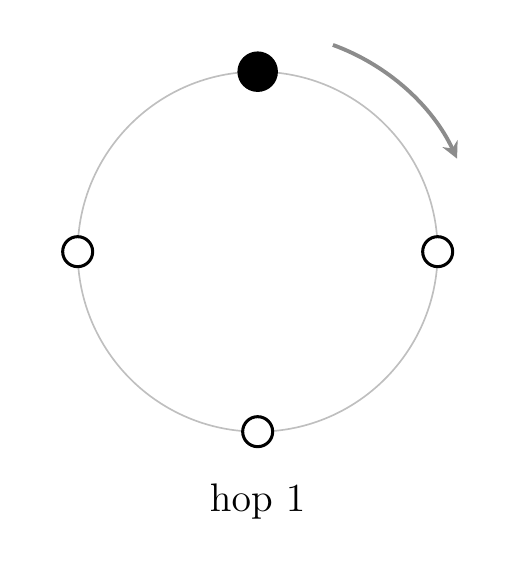
\begin{tikzpicture}[x=1in,y=1in]
\useasboundingbox (-1.15,-1.48) rectangle (1.15,1.12);
\draw[black!25, line width=0.6pt] (0,0) circle (0.9);
\fill[black] (0,0.9) circle (0.1013);
\filldraw[fill=white, draw=black, line width=1.1pt] (0.9,0) circle (0.075);
\filldraw[fill=white, draw=black, line width=1.1pt] (0,-0.9) circle (0.075);
\filldraw[fill=white, draw=black, line width=1.1pt] (-0.9,0) circle (0.075);
\draw[black!45, line width=1.4pt, -{Stealth[length=6pt, width=6pt]}] (0.3762,1.0337) arc[start angle=70, end angle=25, radius=1.1];
\node[font=\Large] at (0,-1.25) {hop 1};
\end{tikzpicture}\hfill 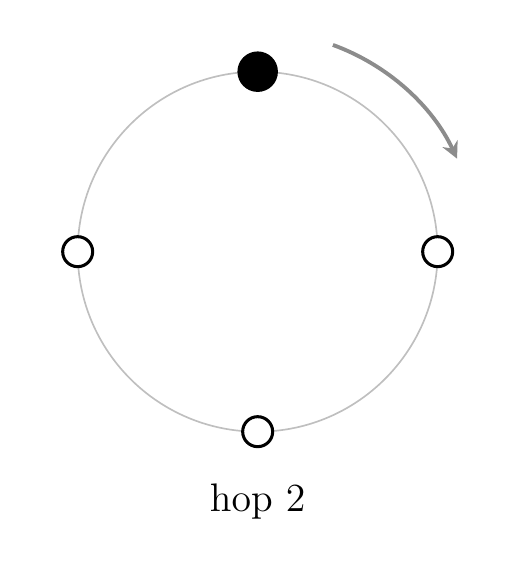
\begin{tikzpicture}[x=1in,y=1in]
\useasboundingbox (-1.15,-1.48) rectangle (1.15,1.12);
\draw[black!25, line width=0.6pt] (0,0) circle (0.9);
\fill[black] (0,0.9) circle (0.1013);
\filldraw[fill=white, draw=black, line width=1.1pt] (0.9,0) circle (0.075);
\filldraw[fill=white, draw=black, line width=1.1pt] (0,-0.9) circle (0.075);
\filldraw[fill=white, draw=black, line width=1.1pt] (-0.9,0) circle (0.075);
\draw[black!45, line width=1.4pt, -{Stealth[length=6pt, width=6pt]}] (0.3762,1.0337) arc[start angle=70, end angle=25, radius=1.1];
\node[font=\Large] at (0,-1.25) {hop 2};
\end{tikzpicture}\hfill 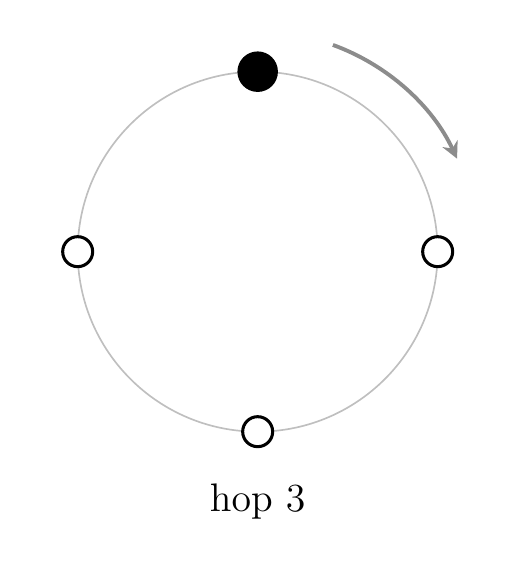
\begin{tikzpicture}[x=1in,y=1in]
\useasboundingbox (-1.15,-1.48) rectangle (1.15,1.12);
\draw[black!25, line width=0.6pt] (0,0) circle (0.9);
\fill[black] (0,0.9) circle (0.1013);
\filldraw[fill=white, draw=black, line width=1.1pt] (0.9,0) circle (0.075);
\filldraw[fill=white, draw=black, line width=1.1pt] (0,-0.9) circle (0.075);
\filldraw[fill=white, draw=black, line width=1.1pt] (-0.9,0) circle (0.075);
\draw[black!45, line width=1.4pt, -{Stealth[length=6pt, width=6pt]}] (0.3762,1.0337) arc[start angle=70, end angle=25, radius=1.1];
\node[font=\Large] at (0,-1.25) {hop 3};
\end{tikzpicture}\hfill}\par
\vfill

\newpage
\par\vspace{0in}\noindent \prob{2} Do the same with this ring of 5 dots.\par
\par\vspace{0.15in}\noindent\makebox[\textwidth][c]{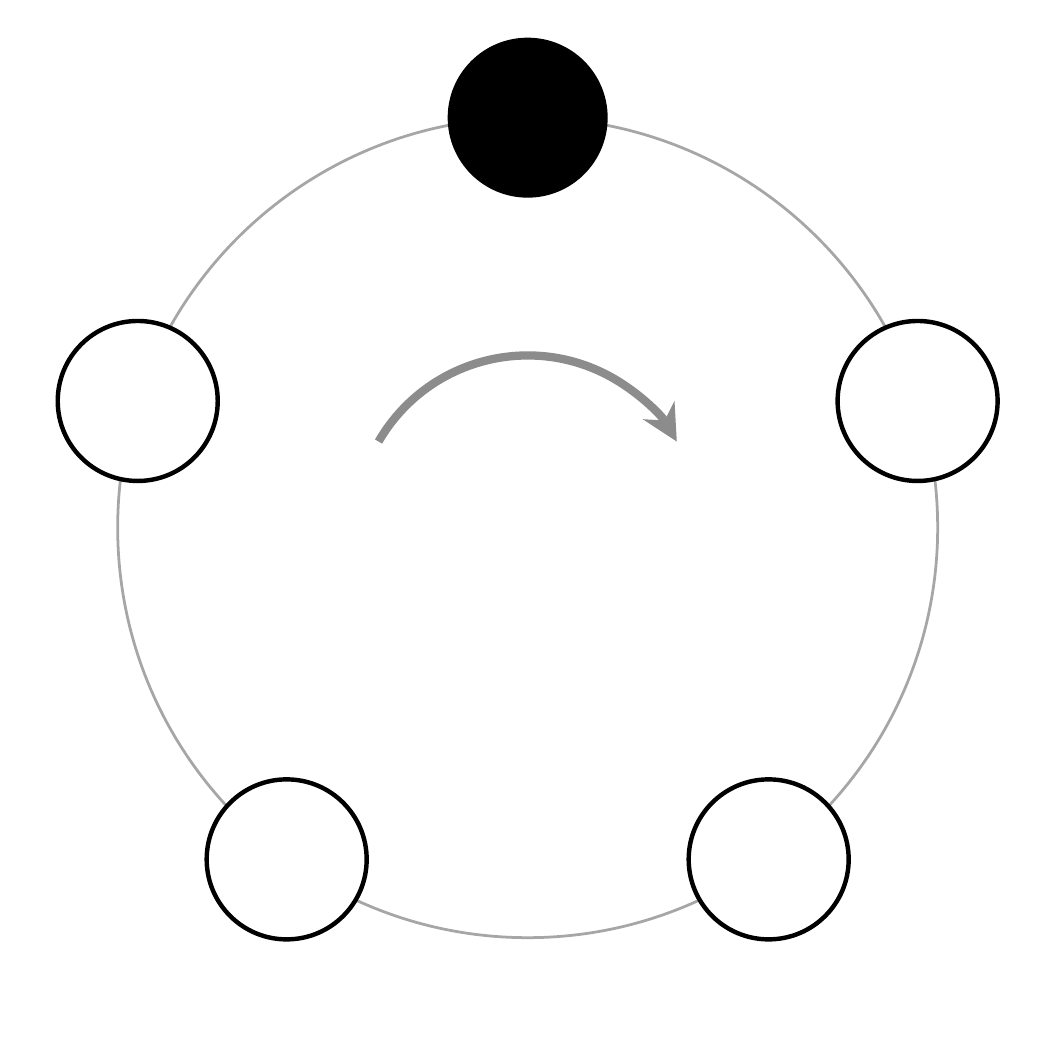
\begin{tikzpicture}[x=1in,y=1in]
\useasboundingbox (-2.5,-2.5) rectangle (2.5,2.5);
\draw[black!35, line width=1pt] (0,0) circle (2.05);
\fill[black] (0,2.05) circle (0.4);
\filldraw[fill=white, draw=black, line width=1.6pt] (1.9497,0.6335) circle (0.4);
\filldraw[fill=white, draw=black, line width=1.6pt] (1.205,-1.6585) circle (0.4);
\filldraw[fill=white, draw=black, line width=1.6pt] (-1.205,-1.6585) circle (0.4);
\filldraw[fill=white, draw=black, line width=1.6pt] (-1.9497,0.6335) circle (0.4);
\draw[black!45, line width=3pt, -{Stealth[length=13pt, width=13pt]}] (-0.7456,0.4305) arc[start angle=150, end angle=30, radius=0.861];
\end{tikzpicture}}\par
\par\vspace{0.15in}\noindent\makebox[\textwidth][s]{\hfill 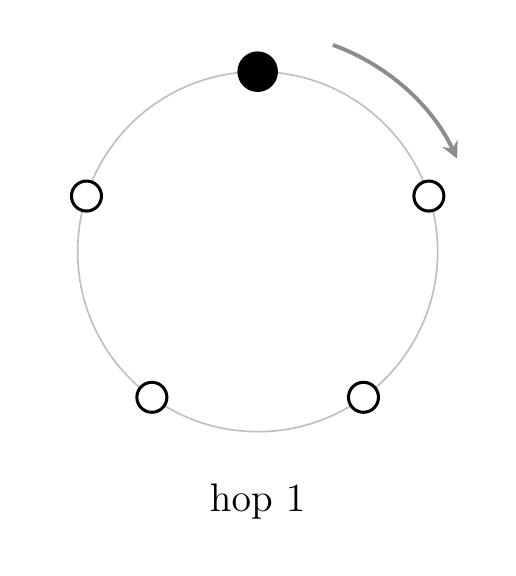
\begin{tikzpicture}[x=1in,y=1in]
\useasboundingbox (-1.15,-1.48) rectangle (1.15,1.12);
\draw[black!25, line width=0.6pt] (0,0) circle (0.9);
\fill[black] (0,0.9) circle (0.1013);
\filldraw[fill=white, draw=black, line width=1.1pt] (0.856,0.2781) circle (0.075);
\filldraw[fill=white, draw=black, line width=1.1pt] (0.529,-0.7281) circle (0.075);
\filldraw[fill=white, draw=black, line width=1.1pt] (-0.529,-0.7281) circle (0.075);
\filldraw[fill=white, draw=black, line width=1.1pt] (-0.856,0.2781) circle (0.075);
\draw[black!45, line width=1.4pt, -{Stealth[length=6pt, width=6pt]}] (0.3762,1.0337) arc[start angle=70, end angle=25, radius=1.1];
\node[font=\Large] at (0,-1.25) {hop 1};
\end{tikzpicture}\hfill 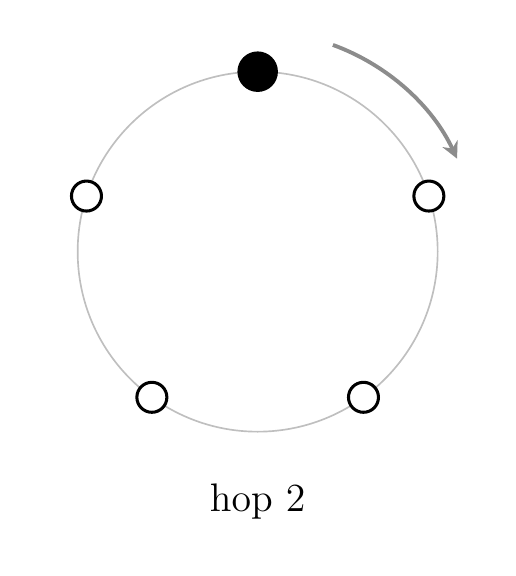
\begin{tikzpicture}[x=1in,y=1in]
\useasboundingbox (-1.15,-1.48) rectangle (1.15,1.12);
\draw[black!25, line width=0.6pt] (0,0) circle (0.9);
\fill[black] (0,0.9) circle (0.1013);
\filldraw[fill=white, draw=black, line width=1.1pt] (0.856,0.2781) circle (0.075);
\filldraw[fill=white, draw=black, line width=1.1pt] (0.529,-0.7281) circle (0.075);
\filldraw[fill=white, draw=black, line width=1.1pt] (-0.529,-0.7281) circle (0.075);
\filldraw[fill=white, draw=black, line width=1.1pt] (-0.856,0.2781) circle (0.075);
\draw[black!45, line width=1.4pt, -{Stealth[length=6pt, width=6pt]}] (0.3762,1.0337) arc[start angle=70, end angle=25, radius=1.1];
\node[font=\Large] at (0,-1.25) {hop 2};
\end{tikzpicture}\hfill 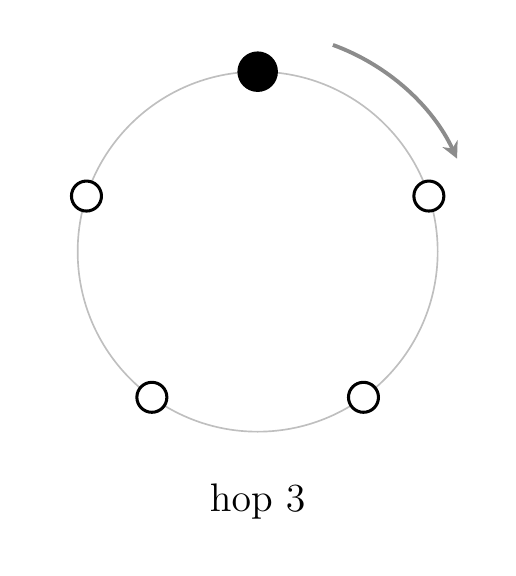
\begin{tikzpicture}[x=1in,y=1in]
\useasboundingbox (-1.15,-1.48) rectangle (1.15,1.12);
\draw[black!25, line width=0.6pt] (0,0) circle (0.9);
\fill[black] (0,0.9) circle (0.1013);
\filldraw[fill=white, draw=black, line width=1.1pt] (0.856,0.2781) circle (0.075);
\filldraw[fill=white, draw=black, line width=1.1pt] (0.529,-0.7281) circle (0.075);
\filldraw[fill=white, draw=black, line width=1.1pt] (-0.529,-0.7281) circle (0.075);
\filldraw[fill=white, draw=black, line width=1.1pt] (-0.856,0.2781) circle (0.075);
\draw[black!45, line width=1.4pt, -{Stealth[length=6pt, width=6pt]}] (0.3762,1.0337) arc[start angle=70, end angle=25, radius=1.1];
\node[font=\Large] at (0,-1.25) {hop 3};
\end{tikzpicture}\hfill}\par
\vfill

\newpage
\par\vspace{0in}\noindent \prob{3} Do the same with this ring of 6 dots.\par
\par\vspace{0.15in}\noindent\makebox[\textwidth][c]{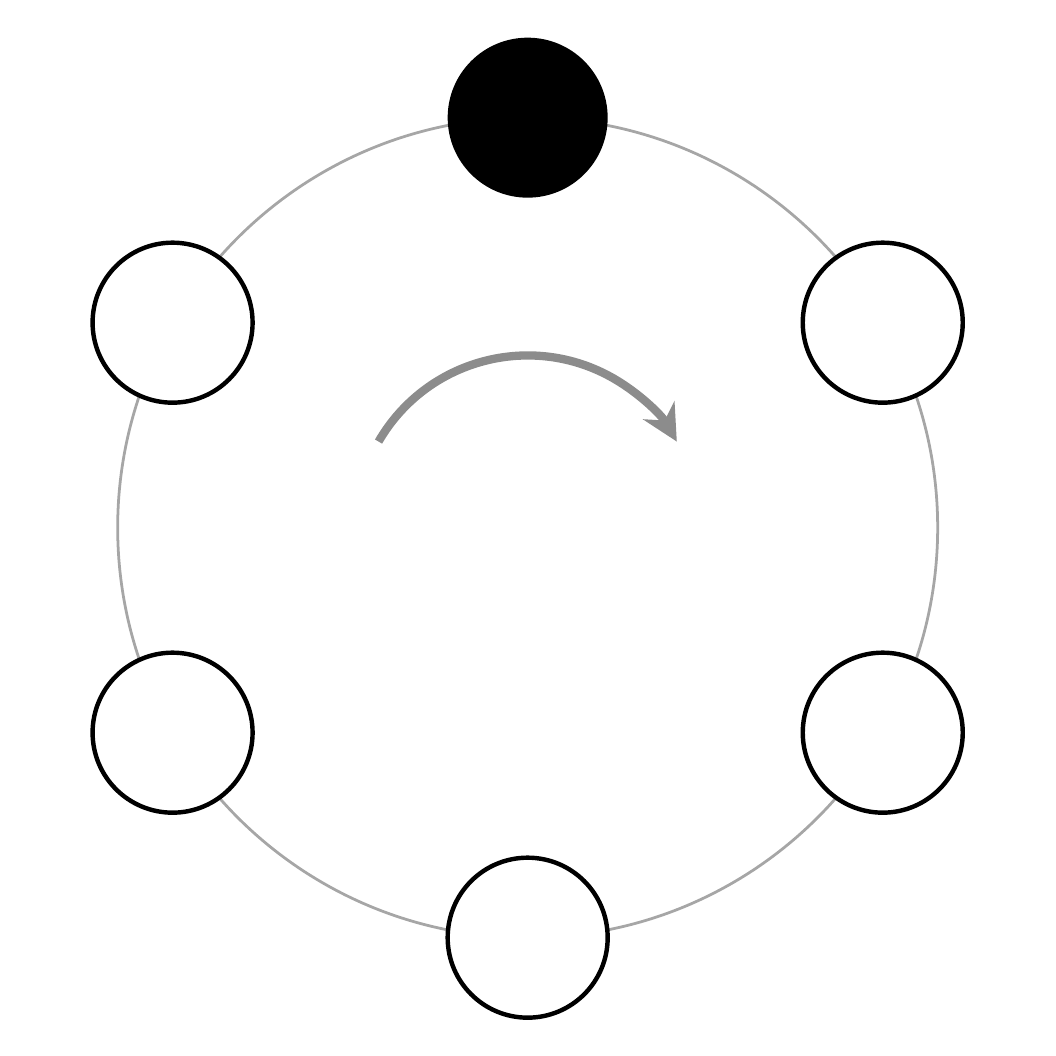
\begin{tikzpicture}[x=1in,y=1in]
\useasboundingbox (-2.5,-2.5) rectangle (2.5,2.5);
\draw[black!35, line width=1pt] (0,0) circle (2.05);
\fill[black] (0,2.05) circle (0.4);
\filldraw[fill=white, draw=black, line width=1.6pt] (1.7754,1.025) circle (0.4);
\filldraw[fill=white, draw=black, line width=1.6pt] (1.7754,-1.025) circle (0.4);
\filldraw[fill=white, draw=black, line width=1.6pt] (0,-2.05) circle (0.4);
\filldraw[fill=white, draw=black, line width=1.6pt] (-1.7754,-1.025) circle (0.4);
\filldraw[fill=white, draw=black, line width=1.6pt] (-1.7754,1.025) circle (0.4);
\draw[black!45, line width=3pt, -{Stealth[length=13pt, width=13pt]}] (-0.7456,0.4305) arc[start angle=150, end angle=30, radius=0.861];
\end{tikzpicture}}\par
\par\vspace{0.15in}\noindent\makebox[\textwidth][s]{\hfill 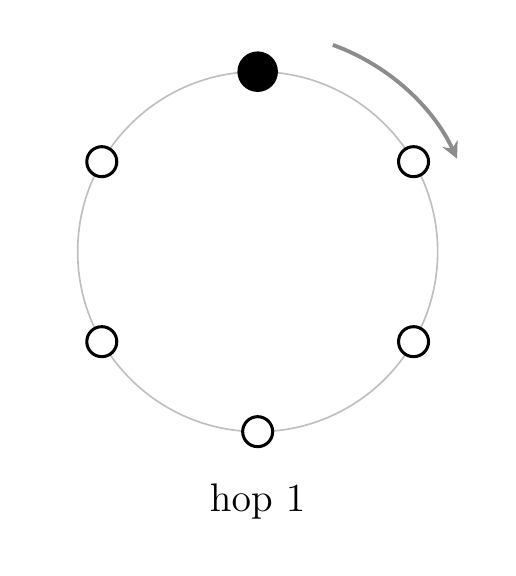
\begin{tikzpicture}[x=1in,y=1in]
\useasboundingbox (-1.15,-1.48) rectangle (1.15,1.12);
\draw[black!25, line width=0.6pt] (0,0) circle (0.9);
\fill[black] (0,0.9) circle (0.1013);
\filldraw[fill=white, draw=black, line width=1.1pt] (0.7794,0.45) circle (0.075);
\filldraw[fill=white, draw=black, line width=1.1pt] (0.7794,-0.45) circle (0.075);
\filldraw[fill=white, draw=black, line width=1.1pt] (0,-0.9) circle (0.075);
\filldraw[fill=white, draw=black, line width=1.1pt] (-0.7794,-0.45) circle (0.075);
\filldraw[fill=white, draw=black, line width=1.1pt] (-0.7794,0.45) circle (0.075);
\draw[black!45, line width=1.4pt, -{Stealth[length=6pt, width=6pt]}] (0.3762,1.0337) arc[start angle=70, end angle=25, radius=1.1];
\node[font=\Large] at (0,-1.25) {hop 1};
\end{tikzpicture}\hfill 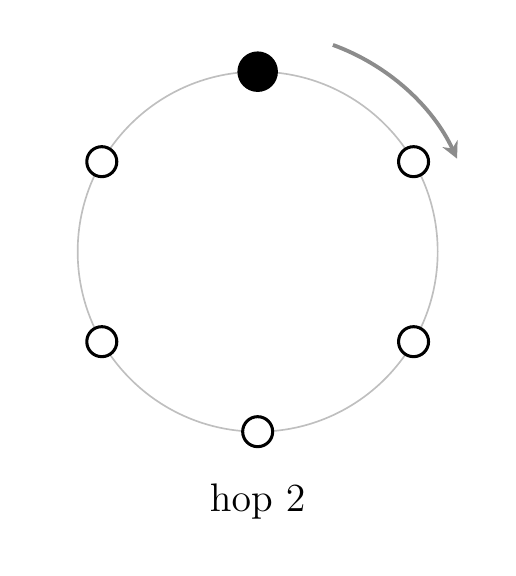
\begin{tikzpicture}[x=1in,y=1in]
\useasboundingbox (-1.15,-1.48) rectangle (1.15,1.12);
\draw[black!25, line width=0.6pt] (0,0) circle (0.9);
\fill[black] (0,0.9) circle (0.1013);
\filldraw[fill=white, draw=black, line width=1.1pt] (0.7794,0.45) circle (0.075);
\filldraw[fill=white, draw=black, line width=1.1pt] (0.7794,-0.45) circle (0.075);
\filldraw[fill=white, draw=black, line width=1.1pt] (0,-0.9) circle (0.075);
\filldraw[fill=white, draw=black, line width=1.1pt] (-0.7794,-0.45) circle (0.075);
\filldraw[fill=white, draw=black, line width=1.1pt] (-0.7794,0.45) circle (0.075);
\draw[black!45, line width=1.4pt, -{Stealth[length=6pt, width=6pt]}] (0.3762,1.0337) arc[start angle=70, end angle=25, radius=1.1];
\node[font=\Large] at (0,-1.25) {hop 2};
\end{tikzpicture}\hfill 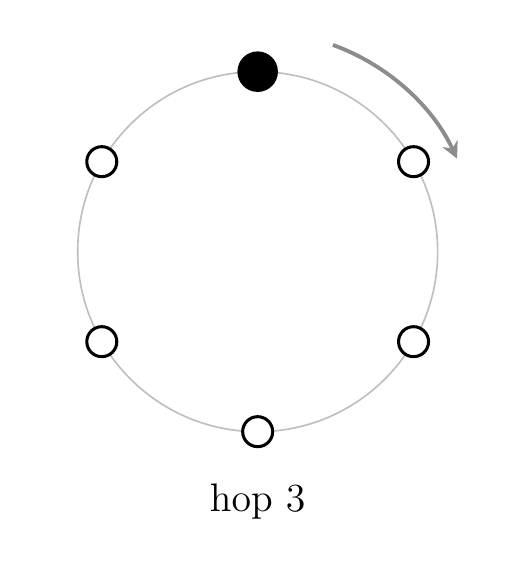
\begin{tikzpicture}[x=1in,y=1in]
\useasboundingbox (-1.15,-1.48) rectangle (1.15,1.12);
\draw[black!25, line width=0.6pt] (0,0) circle (0.9);
\fill[black] (0,0.9) circle (0.1013);
\filldraw[fill=white, draw=black, line width=1.1pt] (0.7794,0.45) circle (0.075);
\filldraw[fill=white, draw=black, line width=1.1pt] (0.7794,-0.45) circle (0.075);
\filldraw[fill=white, draw=black, line width=1.1pt] (0,-0.9) circle (0.075);
\filldraw[fill=white, draw=black, line width=1.1pt] (-0.7794,-0.45) circle (0.075);
\filldraw[fill=white, draw=black, line width=1.1pt] (-0.7794,0.45) circle (0.075);
\draw[black!45, line width=1.4pt, -{Stealth[length=6pt, width=6pt]}] (0.3762,1.0337) arc[start angle=70, end angle=25, radius=1.1];
\node[font=\Large] at (0,-1.25) {hop 3};
\end{tikzpicture}\hfill}\par
\vfill

\newpage
\par\vspace{0in}\noindent \prob{4} Draw the hops from the black dot until you are back. If a dot has no line, start again there with the same hop. Write in the box how many times you started.\par
\par\vspace{0.25in}\noindent\makebox[\textwidth][s]{\hfill \begin{tikzpicture}[x=1in,y=1in]
\useasboundingbox (-1.7,-2.3) rectangle (1.7,1.45);
\draw[black!25, line width=0.6pt] (0,0) circle (1.38);
\fill[black] (0,1.38) circle (0.1148);
\filldraw[fill=white, draw=black, line width=1.1pt] (1.1951,0.69) circle (0.085);
\filldraw[fill=white, draw=black, line width=1.1pt] (1.1951,-0.69) circle (0.085);
\filldraw[fill=white, draw=black, line width=1.1pt] (0,-1.38) circle (0.085);
\filldraw[fill=white, draw=black, line width=1.1pt] (-1.1951,-0.69) circle (0.085);
\filldraw[fill=white, draw=black, line width=1.1pt] (-1.1951,0.69) circle (0.085);
\draw[black!45, line width=1.4pt, -{Stealth[length=6pt, width=6pt]}] (0.5404,1.4847) arc[start angle=70, end angle=25, radius=1.58];
\node[font=\Large, anchor=east] at (0.05,-1.95) {hop 2};
\draw[line width=1pt] (0.345,-2.225) rectangle (0.895,-1.675);
\end{tikzpicture}\hfill \begin{tikzpicture}[x=1in,y=1in]
\useasboundingbox (-1.7,-2.3) rectangle (1.7,1.45);
\draw[black!25, line width=0.6pt] (0,0) circle (1.38);
\fill[black] (0,1.38) circle (0.1148);
\filldraw[fill=white, draw=black, line width=1.1pt] (1.1951,0.69) circle (0.085);
\filldraw[fill=white, draw=black, line width=1.1pt] (1.1951,-0.69) circle (0.085);
\filldraw[fill=white, draw=black, line width=1.1pt] (0,-1.38) circle (0.085);
\filldraw[fill=white, draw=black, line width=1.1pt] (-1.1951,-0.69) circle (0.085);
\filldraw[fill=white, draw=black, line width=1.1pt] (-1.1951,0.69) circle (0.085);
\draw[black!45, line width=1.4pt, -{Stealth[length=6pt, width=6pt]}] (0.5404,1.4847) arc[start angle=70, end angle=25, radius=1.58];
\node[font=\Large, anchor=east] at (0.05,-1.95) {hop 3};
\draw[line width=1pt] (0.345,-2.225) rectangle (0.895,-1.675);
\end{tikzpicture}\hfill}\par
\par\vspace{0.3in}\noindent\makebox[\textwidth][s]{\hfill 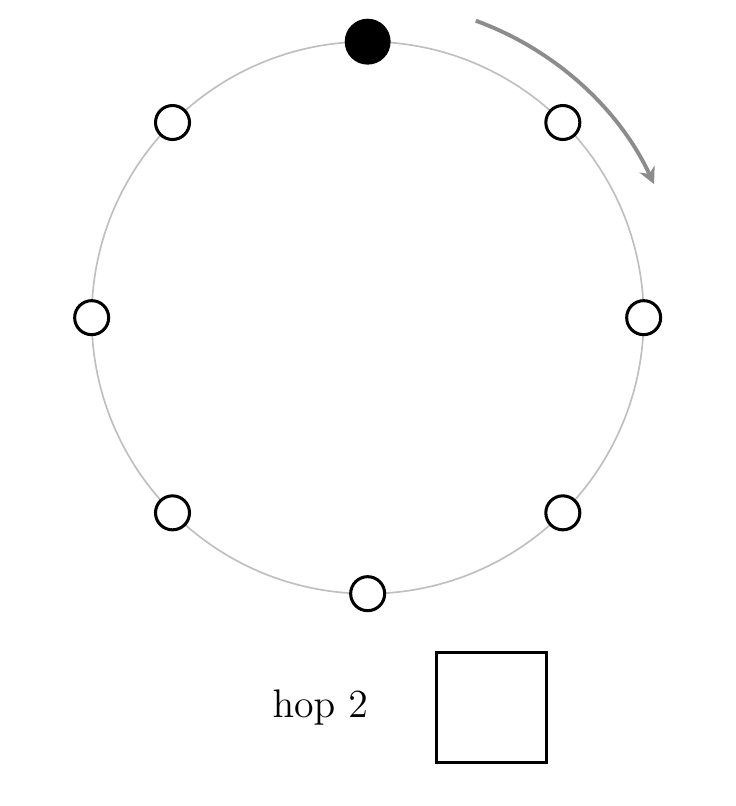
\begin{tikzpicture}[x=1in,y=1in]
\useasboundingbox (-1.7,-2.3) rectangle (1.7,1.45);
\draw[black!25, line width=0.6pt] (0,0) circle (1.38);
\fill[black] (0,1.38) circle (0.1148);
\filldraw[fill=white, draw=black, line width=1.1pt] (0.9758,0.9758) circle (0.085);
\filldraw[fill=white, draw=black, line width=1.1pt] (1.38,0) circle (0.085);
\filldraw[fill=white, draw=black, line width=1.1pt] (0.9758,-0.9758) circle (0.085);
\filldraw[fill=white, draw=black, line width=1.1pt] (0,-1.38) circle (0.085);
\filldraw[fill=white, draw=black, line width=1.1pt] (-0.9758,-0.9758) circle (0.085);
\filldraw[fill=white, draw=black, line width=1.1pt] (-1.38,0) circle (0.085);
\filldraw[fill=white, draw=black, line width=1.1pt] (-0.9758,0.9758) circle (0.085);
\draw[black!45, line width=1.4pt, -{Stealth[length=6pt, width=6pt]}] (0.5404,1.4847) arc[start angle=70, end angle=25, radius=1.58];
\node[font=\Large, anchor=east] at (0.05,-1.95) {hop 2};
\draw[line width=1pt] (0.345,-2.225) rectangle (0.895,-1.675);
\end{tikzpicture}\hfill 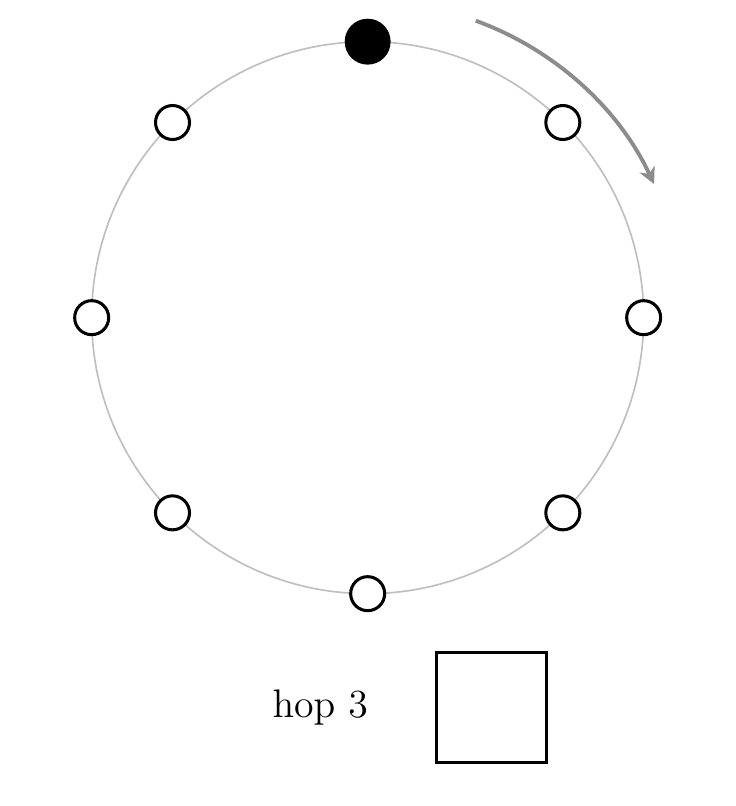
\begin{tikzpicture}[x=1in,y=1in]
\useasboundingbox (-1.7,-2.3) rectangle (1.7,1.45);
\draw[black!25, line width=0.6pt] (0,0) circle (1.38);
\fill[black] (0,1.38) circle (0.1148);
\filldraw[fill=white, draw=black, line width=1.1pt] (0.9758,0.9758) circle (0.085);
\filldraw[fill=white, draw=black, line width=1.1pt] (1.38,0) circle (0.085);
\filldraw[fill=white, draw=black, line width=1.1pt] (0.9758,-0.9758) circle (0.085);
\filldraw[fill=white, draw=black, line width=1.1pt] (0,-1.38) circle (0.085);
\filldraw[fill=white, draw=black, line width=1.1pt] (-0.9758,-0.9758) circle (0.085);
\filldraw[fill=white, draw=black, line width=1.1pt] (-1.38,0) circle (0.085);
\filldraw[fill=white, draw=black, line width=1.1pt] (-0.9758,0.9758) circle (0.085);
\draw[black!45, line width=1.4pt, -{Stealth[length=6pt, width=6pt]}] (0.5404,1.4847) arc[start angle=70, end angle=25, radius=1.58];
\node[font=\Large, anchor=east] at (0.05,-1.95) {hop 3};
\draw[line width=1pt] (0.345,-2.225) rectangle (0.895,-1.675);
\end{tikzpicture}\hfill}\par
\vfill

\newpage
\par\vspace{0in}\noindent \prob{5} Find every hop from 1 to 5 that draws each picture. Write the hops under the picture.\par
\par\vspace{0.3in}\noindent\makebox[\textwidth][s]{\hfill 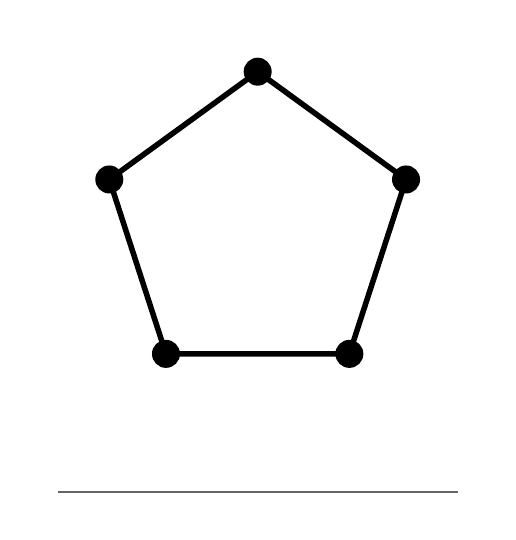
\begin{tikzpicture}[x=1in,y=1in]
\useasboundingbox (-1.15,-1.42) rectangle (1.15,1);
\draw[black, line width=2pt, line join=round] (0,0.78) -- (0.7418,0.241) -- (0.4585,-0.631) -- (-0.4585,-0.631) -- (-0.7418,0.241) -- cycle;
\fill (0,0.78) circle (0.07);
\fill (0.7418,0.241) circle (0.07);
\fill (0.4585,-0.631) circle (0.07);
\fill (-0.4585,-0.631) circle (0.07);
\fill (-0.7418,0.241) circle (0.07);
\draw[black!60, line width=0.8pt] (-1,-1.32) -- (1,-1.32);
\end{tikzpicture}\hfill 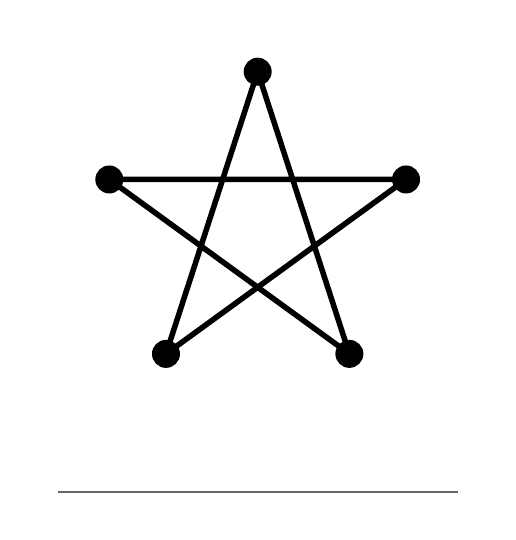
\begin{tikzpicture}[x=1in,y=1in]
\useasboundingbox (-1.15,-1.42) rectangle (1.15,1);
\draw[black, line width=2pt, line join=round] (0,0.78) -- (0.4585,-0.631) -- (-0.7418,0.241) -- (0.7418,0.241) -- (-0.4585,-0.631) -- cycle;
\fill (0,0.78) circle (0.07);
\fill (0.7418,0.241) circle (0.07);
\fill (0.4585,-0.631) circle (0.07);
\fill (-0.4585,-0.631) circle (0.07);
\fill (-0.7418,0.241) circle (0.07);
\draw[black!60, line width=0.8pt] (-1,-1.32) -- (1,-1.32);
\end{tikzpicture}\hfill 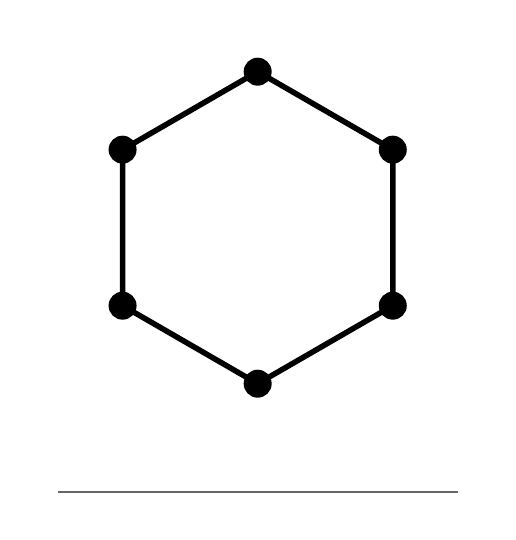
\begin{tikzpicture}[x=1in,y=1in]
\useasboundingbox (-1.15,-1.42) rectangle (1.15,1);
\draw[black, line width=2pt, line join=round] (0,0.78) -- (0.6755,0.39) -- (0.6755,-0.39) -- (0,-0.78) -- (-0.6755,-0.39) -- (-0.6755,0.39) -- cycle;
\fill (0,0.78) circle (0.07);
\fill (0.6755,0.39) circle (0.07);
\fill (0.6755,-0.39) circle (0.07);
\fill (0,-0.78) circle (0.07);
\fill (-0.6755,-0.39) circle (0.07);
\fill (-0.6755,0.39) circle (0.07);
\draw[black!60, line width=0.8pt] (-1,-1.32) -- (1,-1.32);
\end{tikzpicture}\hfill}\par
\par\vspace{0.3in}\noindent\makebox[\textwidth][s]{\hfill \hspace{0.6in}\hfill 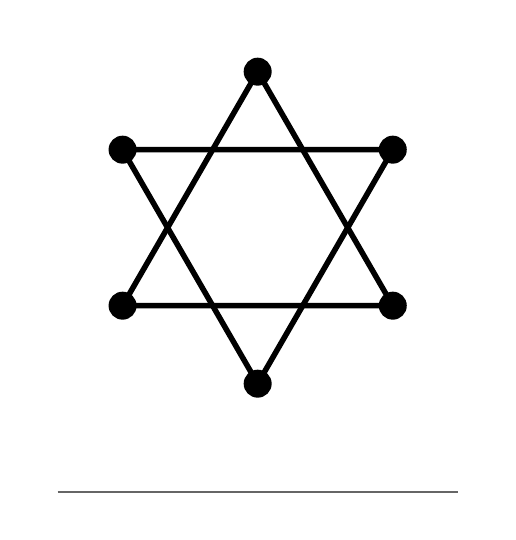
\begin{tikzpicture}[x=1in,y=1in]
\useasboundingbox (-1.15,-1.42) rectangle (1.15,1);
\draw[black, line width=2pt, line join=round] (0,0.78) -- (0.6755,-0.39) -- (-0.6755,-0.39) -- cycle;
\draw[black, line width=2pt, line join=round] (0.6755,0.39) -- (0,-0.78) -- (-0.6755,0.39) -- cycle;
\fill (0,0.78) circle (0.07);
\fill (0.6755,0.39) circle (0.07);
\fill (0.6755,-0.39) circle (0.07);
\fill (0,-0.78) circle (0.07);
\fill (-0.6755,-0.39) circle (0.07);
\fill (-0.6755,0.39) circle (0.07);
\draw[black!60, line width=0.8pt] (-1,-1.32) -- (1,-1.32);
\end{tikzpicture}\hfill 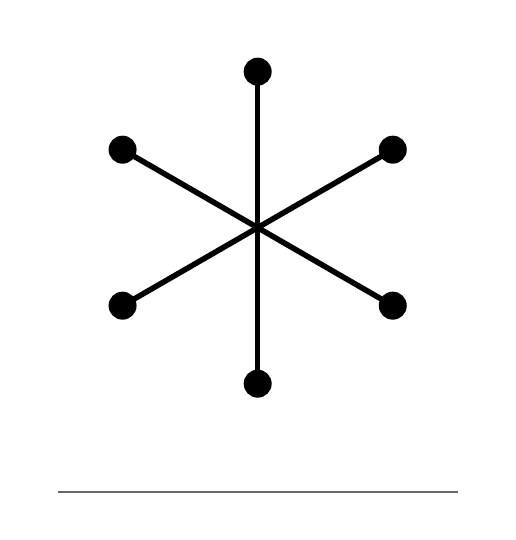
\begin{tikzpicture}[x=1in,y=1in]
\useasboundingbox (-1.15,-1.42) rectangle (1.15,1);
\draw[black, line width=2pt] (0,0.78) -- (0,-0.78);
\draw[black, line width=2pt] (0.6755,0.39) -- (-0.6755,-0.39);
\draw[black, line width=2pt] (0.6755,-0.39) -- (-0.6755,0.39);
\fill (0,0.78) circle (0.07);
\fill (0.6755,0.39) circle (0.07);
\fill (0.6755,-0.39) circle (0.07);
\fill (0,-0.78) circle (0.07);
\fill (-0.6755,-0.39) circle (0.07);
\fill (-0.6755,0.39) circle (0.07);
\draw[black!60, line width=0.8pt] (-1,-1.32) -- (1,-1.32);
\end{tikzpicture}\hfill \hspace{0.6in}\hfill}\par
\par\vspace{0.45in}\noindent\makebox[\textwidth][s]{\hfill 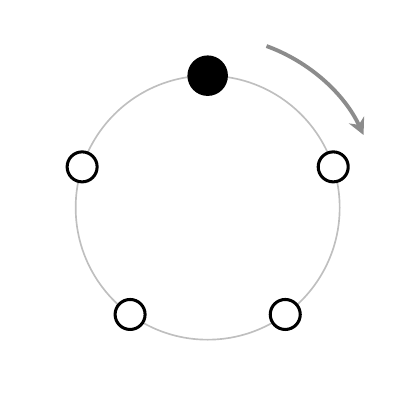
\begin{tikzpicture}[x=1in,y=1in]
\useasboundingbox (-0.9,-0.82) rectangle (0.9,0.9);
\draw[black!25, line width=0.6pt] (0,0) circle (0.66);
\fill[black] (0,0.66) circle (0.1013);
\filldraw[fill=white, draw=black, line width=1.1pt] (0.6277,0.204) circle (0.075);
\filldraw[fill=white, draw=black, line width=1.1pt] (0.3879,-0.534) circle (0.075);
\filldraw[fill=white, draw=black, line width=1.1pt] (-0.3879,-0.534) circle (0.075);
\filldraw[fill=white, draw=black, line width=1.1pt] (-0.6277,0.204) circle (0.075);
\draw[black!45, line width=1.4pt, -{Stealth[length=6pt, width=6pt]}] (0.2941,0.8081) arc[start angle=70, end angle=25, radius=0.86];
\end{tikzpicture}\hfill 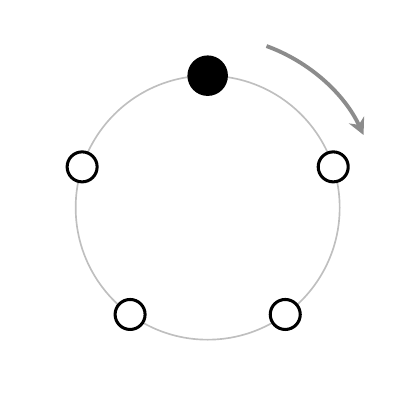
\begin{tikzpicture}[x=1in,y=1in]
\useasboundingbox (-0.9,-0.82) rectangle (0.9,0.9);
\draw[black!25, line width=0.6pt] (0,0) circle (0.66);
\fill[black] (0,0.66) circle (0.1013);
\filldraw[fill=white, draw=black, line width=1.1pt] (0.6277,0.204) circle (0.075);
\filldraw[fill=white, draw=black, line width=1.1pt] (0.3879,-0.534) circle (0.075);
\filldraw[fill=white, draw=black, line width=1.1pt] (-0.3879,-0.534) circle (0.075);
\filldraw[fill=white, draw=black, line width=1.1pt] (-0.6277,0.204) circle (0.075);
\draw[black!45, line width=1.4pt, -{Stealth[length=6pt, width=6pt]}] (0.2941,0.8081) arc[start angle=70, end angle=25, radius=0.86];
\end{tikzpicture}\hfill 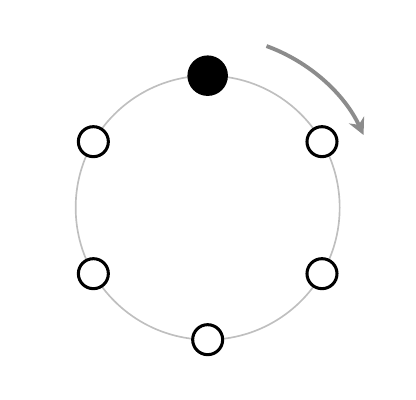
\begin{tikzpicture}[x=1in,y=1in]
\useasboundingbox (-0.9,-0.82) rectangle (0.9,0.9);
\draw[black!25, line width=0.6pt] (0,0) circle (0.66);
\fill[black] (0,0.66) circle (0.1013);
\filldraw[fill=white, draw=black, line width=1.1pt] (0.5716,0.33) circle (0.075);
\filldraw[fill=white, draw=black, line width=1.1pt] (0.5716,-0.33) circle (0.075);
\filldraw[fill=white, draw=black, line width=1.1pt] (0,-0.66) circle (0.075);
\filldraw[fill=white, draw=black, line width=1.1pt] (-0.5716,-0.33) circle (0.075);
\filldraw[fill=white, draw=black, line width=1.1pt] (-0.5716,0.33) circle (0.075);
\draw[black!45, line width=1.4pt, -{Stealth[length=6pt, width=6pt]}] (0.2941,0.8081) arc[start angle=70, end angle=25, radius=0.86];
\end{tikzpicture}\hfill 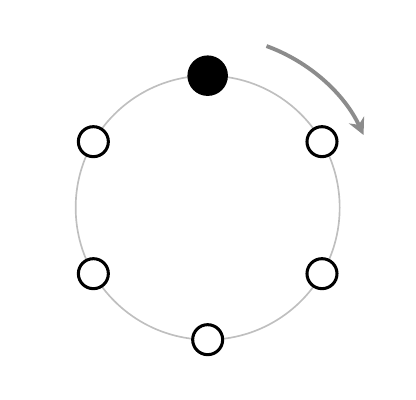
\begin{tikzpicture}[x=1in,y=1in]
\useasboundingbox (-0.9,-0.82) rectangle (0.9,0.9);
\draw[black!25, line width=0.6pt] (0,0) circle (0.66);
\fill[black] (0,0.66) circle (0.1013);
\filldraw[fill=white, draw=black, line width=1.1pt] (0.5716,0.33) circle (0.075);
\filldraw[fill=white, draw=black, line width=1.1pt] (0.5716,-0.33) circle (0.075);
\filldraw[fill=white, draw=black, line width=1.1pt] (0,-0.66) circle (0.075);
\filldraw[fill=white, draw=black, line width=1.1pt] (-0.5716,-0.33) circle (0.075);
\filldraw[fill=white, draw=black, line width=1.1pt] (-0.5716,0.33) circle (0.075);
\draw[black!45, line width=1.4pt, -{Stealth[length=6pt, width=6pt]}] (0.2941,0.8081) arc[start angle=70, end angle=25, radius=0.86];
\end{tikzpicture}\hfill}\par
\vfill

\newpage
\par\vspace{0in}\noindent \prob{6} Put a counter on the black dot and hop it until it is back. Draw each hop on a small ring, and circle each hop that lands on every dot.\par
\par\vspace{0.15in}\noindent\makebox[\textwidth][c]{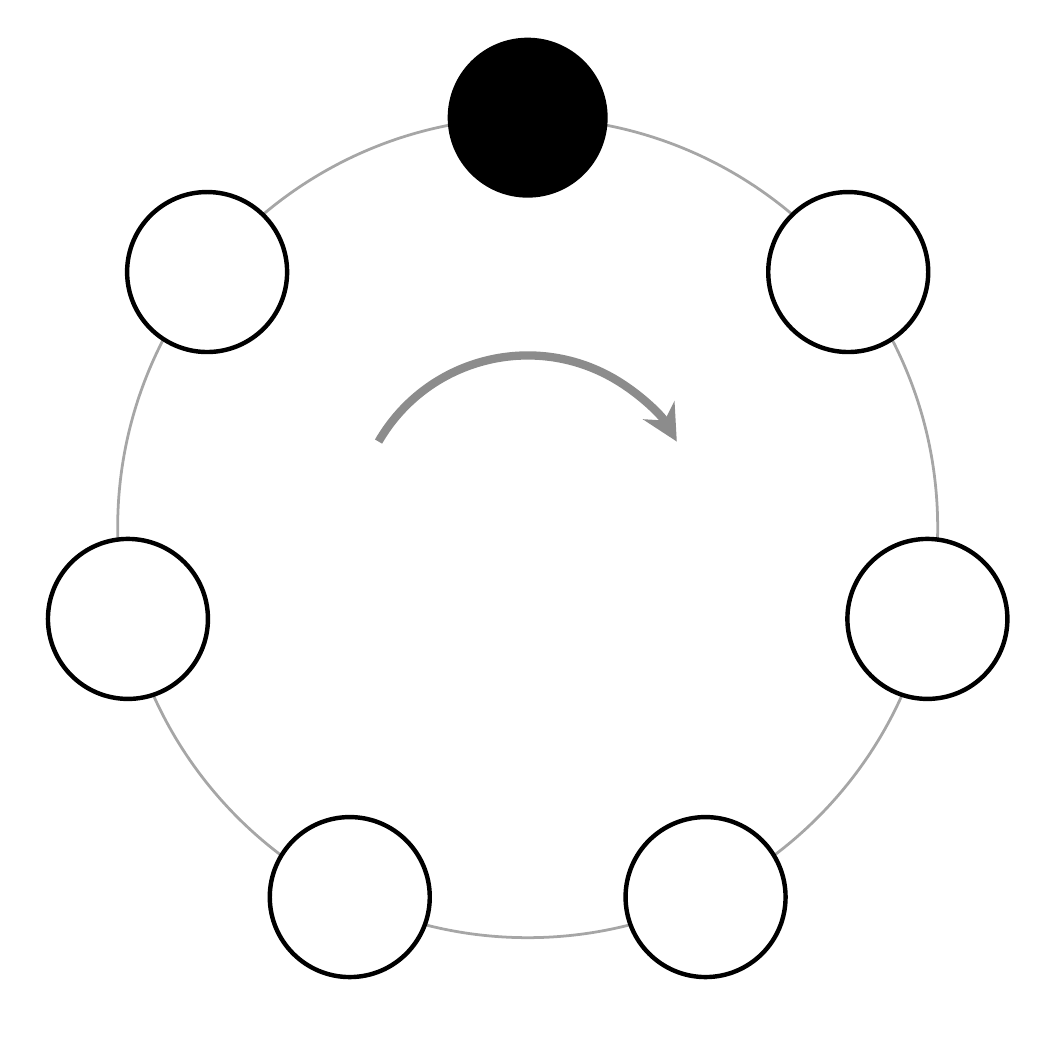
\begin{tikzpicture}[x=1in,y=1in]
\useasboundingbox (-2.5,-2.5) rectangle (2.5,2.5);
\draw[black!35, line width=1pt] (0,0) circle (2.05);
\fill[black] (0,2.05) circle (0.4);
\filldraw[fill=white, draw=black, line width=1.6pt] (1.6028,1.2782) circle (0.4);
\filldraw[fill=white, draw=black, line width=1.6pt] (1.9986,-0.4562) circle (0.4);
\filldraw[fill=white, draw=black, line width=1.6pt] (0.8895,-1.847) circle (0.4);
\filldraw[fill=white, draw=black, line width=1.6pt] (-0.8895,-1.847) circle (0.4);
\filldraw[fill=white, draw=black, line width=1.6pt] (-1.9986,-0.4562) circle (0.4);
\filldraw[fill=white, draw=black, line width=1.6pt] (-1.6028,1.2782) circle (0.4);
\draw[black!45, line width=3pt, -{Stealth[length=13pt, width=13pt]}] (-0.7456,0.4305) arc[start angle=150, end angle=30, radius=0.861];
\end{tikzpicture}}\par
\par\vspace{0.15in}\noindent\makebox[\textwidth][s]{\hfill 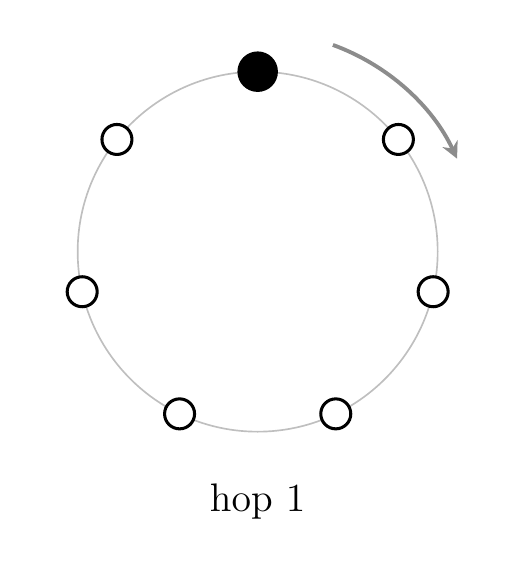
\begin{tikzpicture}[x=1in,y=1in]
\useasboundingbox (-1.15,-1.48) rectangle (1.15,1.12);
\draw[black!25, line width=0.6pt] (0,0) circle (0.9);
\fill[black] (0,0.9) circle (0.1013);
\filldraw[fill=white, draw=black, line width=1.1pt] (0.7036,0.5611) circle (0.075);
\filldraw[fill=white, draw=black, line width=1.1pt] (0.8774,-0.2003) circle (0.075);
\filldraw[fill=white, draw=black, line width=1.1pt] (0.3905,-0.8109) circle (0.075);
\filldraw[fill=white, draw=black, line width=1.1pt] (-0.3905,-0.8109) circle (0.075);
\filldraw[fill=white, draw=black, line width=1.1pt] (-0.8774,-0.2003) circle (0.075);
\filldraw[fill=white, draw=black, line width=1.1pt] (-0.7036,0.5611) circle (0.075);
\draw[black!45, line width=1.4pt, -{Stealth[length=6pt, width=6pt]}] (0.3762,1.0337) arc[start angle=70, end angle=25, radius=1.1];
\node[font=\Large] at (0,-1.25) {hop 1};
\end{tikzpicture}\hfill 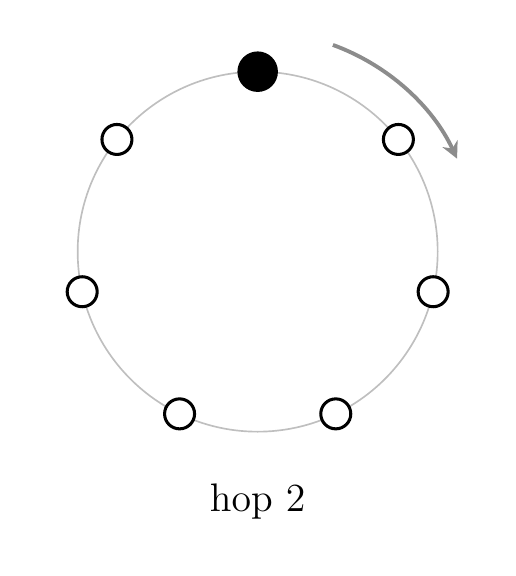
\begin{tikzpicture}[x=1in,y=1in]
\useasboundingbox (-1.15,-1.48) rectangle (1.15,1.12);
\draw[black!25, line width=0.6pt] (0,0) circle (0.9);
\fill[black] (0,0.9) circle (0.1013);
\filldraw[fill=white, draw=black, line width=1.1pt] (0.7036,0.5611) circle (0.075);
\filldraw[fill=white, draw=black, line width=1.1pt] (0.8774,-0.2003) circle (0.075);
\filldraw[fill=white, draw=black, line width=1.1pt] (0.3905,-0.8109) circle (0.075);
\filldraw[fill=white, draw=black, line width=1.1pt] (-0.3905,-0.8109) circle (0.075);
\filldraw[fill=white, draw=black, line width=1.1pt] (-0.8774,-0.2003) circle (0.075);
\filldraw[fill=white, draw=black, line width=1.1pt] (-0.7036,0.5611) circle (0.075);
\draw[black!45, line width=1.4pt, -{Stealth[length=6pt, width=6pt]}] (0.3762,1.0337) arc[start angle=70, end angle=25, radius=1.1];
\node[font=\Large] at (0,-1.25) {hop 2};
\end{tikzpicture}\hfill 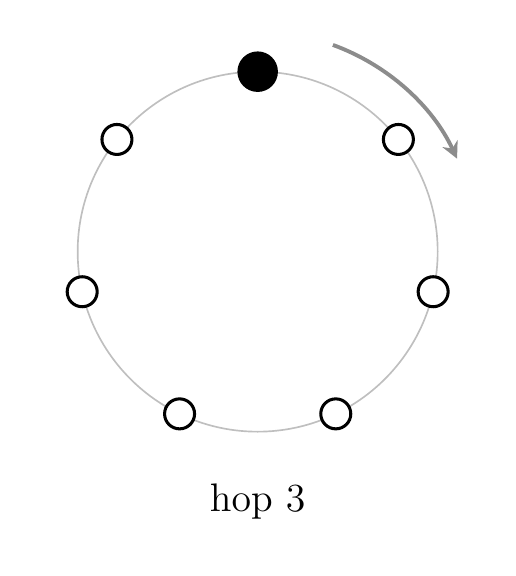
\begin{tikzpicture}[x=1in,y=1in]
\useasboundingbox (-1.15,-1.48) rectangle (1.15,1.12);
\draw[black!25, line width=0.6pt] (0,0) circle (0.9);
\fill[black] (0,0.9) circle (0.1013);
\filldraw[fill=white, draw=black, line width=1.1pt] (0.7036,0.5611) circle (0.075);
\filldraw[fill=white, draw=black, line width=1.1pt] (0.8774,-0.2003) circle (0.075);
\filldraw[fill=white, draw=black, line width=1.1pt] (0.3905,-0.8109) circle (0.075);
\filldraw[fill=white, draw=black, line width=1.1pt] (-0.3905,-0.8109) circle (0.075);
\filldraw[fill=white, draw=black, line width=1.1pt] (-0.8774,-0.2003) circle (0.075);
\filldraw[fill=white, draw=black, line width=1.1pt] (-0.7036,0.5611) circle (0.075);
\draw[black!45, line width=1.4pt, -{Stealth[length=6pt, width=6pt]}] (0.3762,1.0337) arc[start angle=70, end angle=25, radius=1.1];
\node[font=\Large] at (0,-1.25) {hop 3};
\end{tikzpicture}\hfill}\par
\vfill

\newpage
\par\vspace{0in}\noindent \prob{7} Do the same with hop 4, hop 5 and hop 6 on this ring of 7 dots.\par
\par\vspace{0.15in}\noindent\makebox[\textwidth][c]{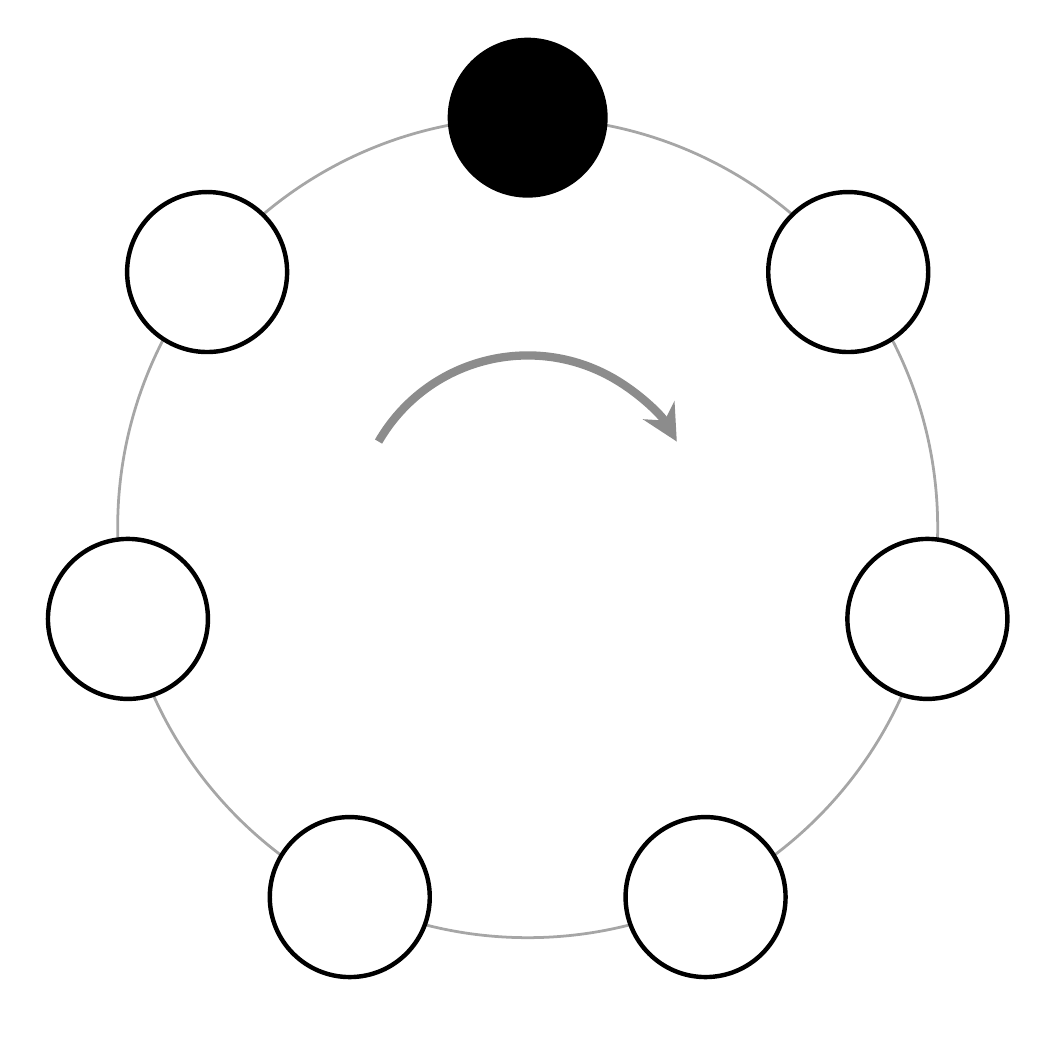
\begin{tikzpicture}[x=1in,y=1in]
\useasboundingbox (-2.5,-2.5) rectangle (2.5,2.5);
\draw[black!35, line width=1pt] (0,0) circle (2.05);
\fill[black] (0,2.05) circle (0.4);
\filldraw[fill=white, draw=black, line width=1.6pt] (1.6028,1.2782) circle (0.4);
\filldraw[fill=white, draw=black, line width=1.6pt] (1.9986,-0.4562) circle (0.4);
\filldraw[fill=white, draw=black, line width=1.6pt] (0.8895,-1.847) circle (0.4);
\filldraw[fill=white, draw=black, line width=1.6pt] (-0.8895,-1.847) circle (0.4);
\filldraw[fill=white, draw=black, line width=1.6pt] (-1.9986,-0.4562) circle (0.4);
\filldraw[fill=white, draw=black, line width=1.6pt] (-1.6028,1.2782) circle (0.4);
\draw[black!45, line width=3pt, -{Stealth[length=13pt, width=13pt]}] (-0.7456,0.4305) arc[start angle=150, end angle=30, radius=0.861];
\end{tikzpicture}}\par
\par\vspace{0.15in}\noindent\makebox[\textwidth][s]{\hfill 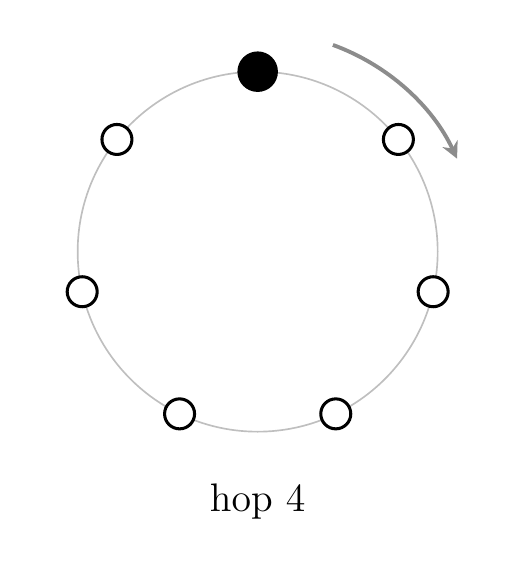
\begin{tikzpicture}[x=1in,y=1in]
\useasboundingbox (-1.15,-1.48) rectangle (1.15,1.12);
\draw[black!25, line width=0.6pt] (0,0) circle (0.9);
\fill[black] (0,0.9) circle (0.1013);
\filldraw[fill=white, draw=black, line width=1.1pt] (0.7036,0.5611) circle (0.075);
\filldraw[fill=white, draw=black, line width=1.1pt] (0.8774,-0.2003) circle (0.075);
\filldraw[fill=white, draw=black, line width=1.1pt] (0.3905,-0.8109) circle (0.075);
\filldraw[fill=white, draw=black, line width=1.1pt] (-0.3905,-0.8109) circle (0.075);
\filldraw[fill=white, draw=black, line width=1.1pt] (-0.8774,-0.2003) circle (0.075);
\filldraw[fill=white, draw=black, line width=1.1pt] (-0.7036,0.5611) circle (0.075);
\draw[black!45, line width=1.4pt, -{Stealth[length=6pt, width=6pt]}] (0.3762,1.0337) arc[start angle=70, end angle=25, radius=1.1];
\node[font=\Large] at (0,-1.25) {hop 4};
\end{tikzpicture}\hfill 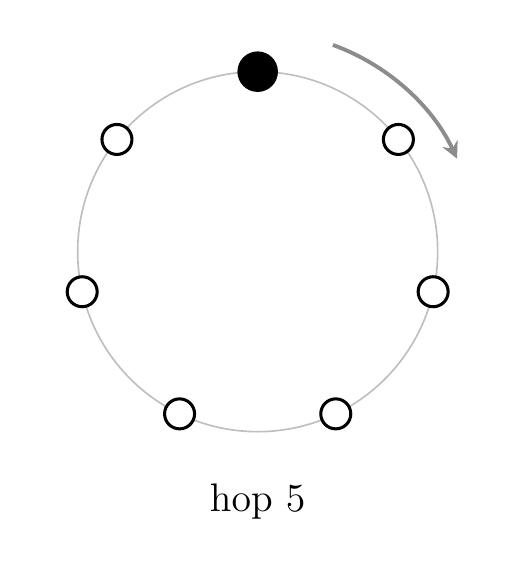
\begin{tikzpicture}[x=1in,y=1in]
\useasboundingbox (-1.15,-1.48) rectangle (1.15,1.12);
\draw[black!25, line width=0.6pt] (0,0) circle (0.9);
\fill[black] (0,0.9) circle (0.1013);
\filldraw[fill=white, draw=black, line width=1.1pt] (0.7036,0.5611) circle (0.075);
\filldraw[fill=white, draw=black, line width=1.1pt] (0.8774,-0.2003) circle (0.075);
\filldraw[fill=white, draw=black, line width=1.1pt] (0.3905,-0.8109) circle (0.075);
\filldraw[fill=white, draw=black, line width=1.1pt] (-0.3905,-0.8109) circle (0.075);
\filldraw[fill=white, draw=black, line width=1.1pt] (-0.8774,-0.2003) circle (0.075);
\filldraw[fill=white, draw=black, line width=1.1pt] (-0.7036,0.5611) circle (0.075);
\draw[black!45, line width=1.4pt, -{Stealth[length=6pt, width=6pt]}] (0.3762,1.0337) arc[start angle=70, end angle=25, radius=1.1];
\node[font=\Large] at (0,-1.25) {hop 5};
\end{tikzpicture}\hfill 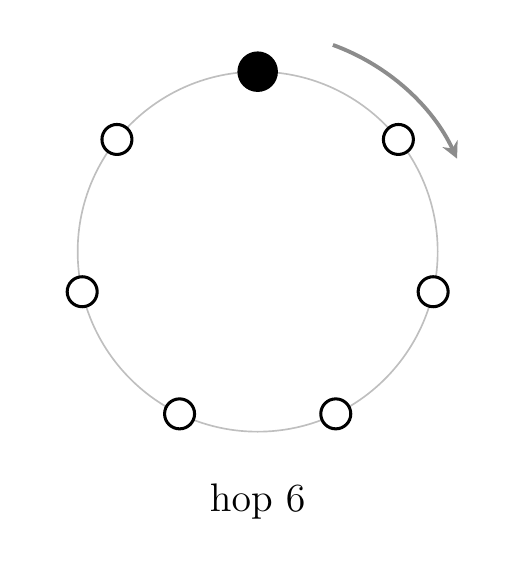
\begin{tikzpicture}[x=1in,y=1in]
\useasboundingbox (-1.15,-1.48) rectangle (1.15,1.12);
\draw[black!25, line width=0.6pt] (0,0) circle (0.9);
\fill[black] (0,0.9) circle (0.1013);
\filldraw[fill=white, draw=black, line width=1.1pt] (0.7036,0.5611) circle (0.075);
\filldraw[fill=white, draw=black, line width=1.1pt] (0.8774,-0.2003) circle (0.075);
\filldraw[fill=white, draw=black, line width=1.1pt] (0.3905,-0.8109) circle (0.075);
\filldraw[fill=white, draw=black, line width=1.1pt] (-0.3905,-0.8109) circle (0.075);
\filldraw[fill=white, draw=black, line width=1.1pt] (-0.8774,-0.2003) circle (0.075);
\filldraw[fill=white, draw=black, line width=1.1pt] (-0.7036,0.5611) circle (0.075);
\draw[black!45, line width=1.4pt, -{Stealth[length=6pt, width=6pt]}] (0.3762,1.0337) arc[start angle=70, end angle=25, radius=1.1];
\node[font=\Large] at (0,-1.25) {hop 6};
\end{tikzpicture}\hfill}\par
\vfill

\newpage
\par\vspace{0in}\noindent \prob{8} Hop 2 changes each picture into the picture 2 places along the arrow. Use hop 2 on each row to make the next row, until you get the top row again.\par
\par\vspace{0.3in}\noindent\makebox[\textwidth][c]{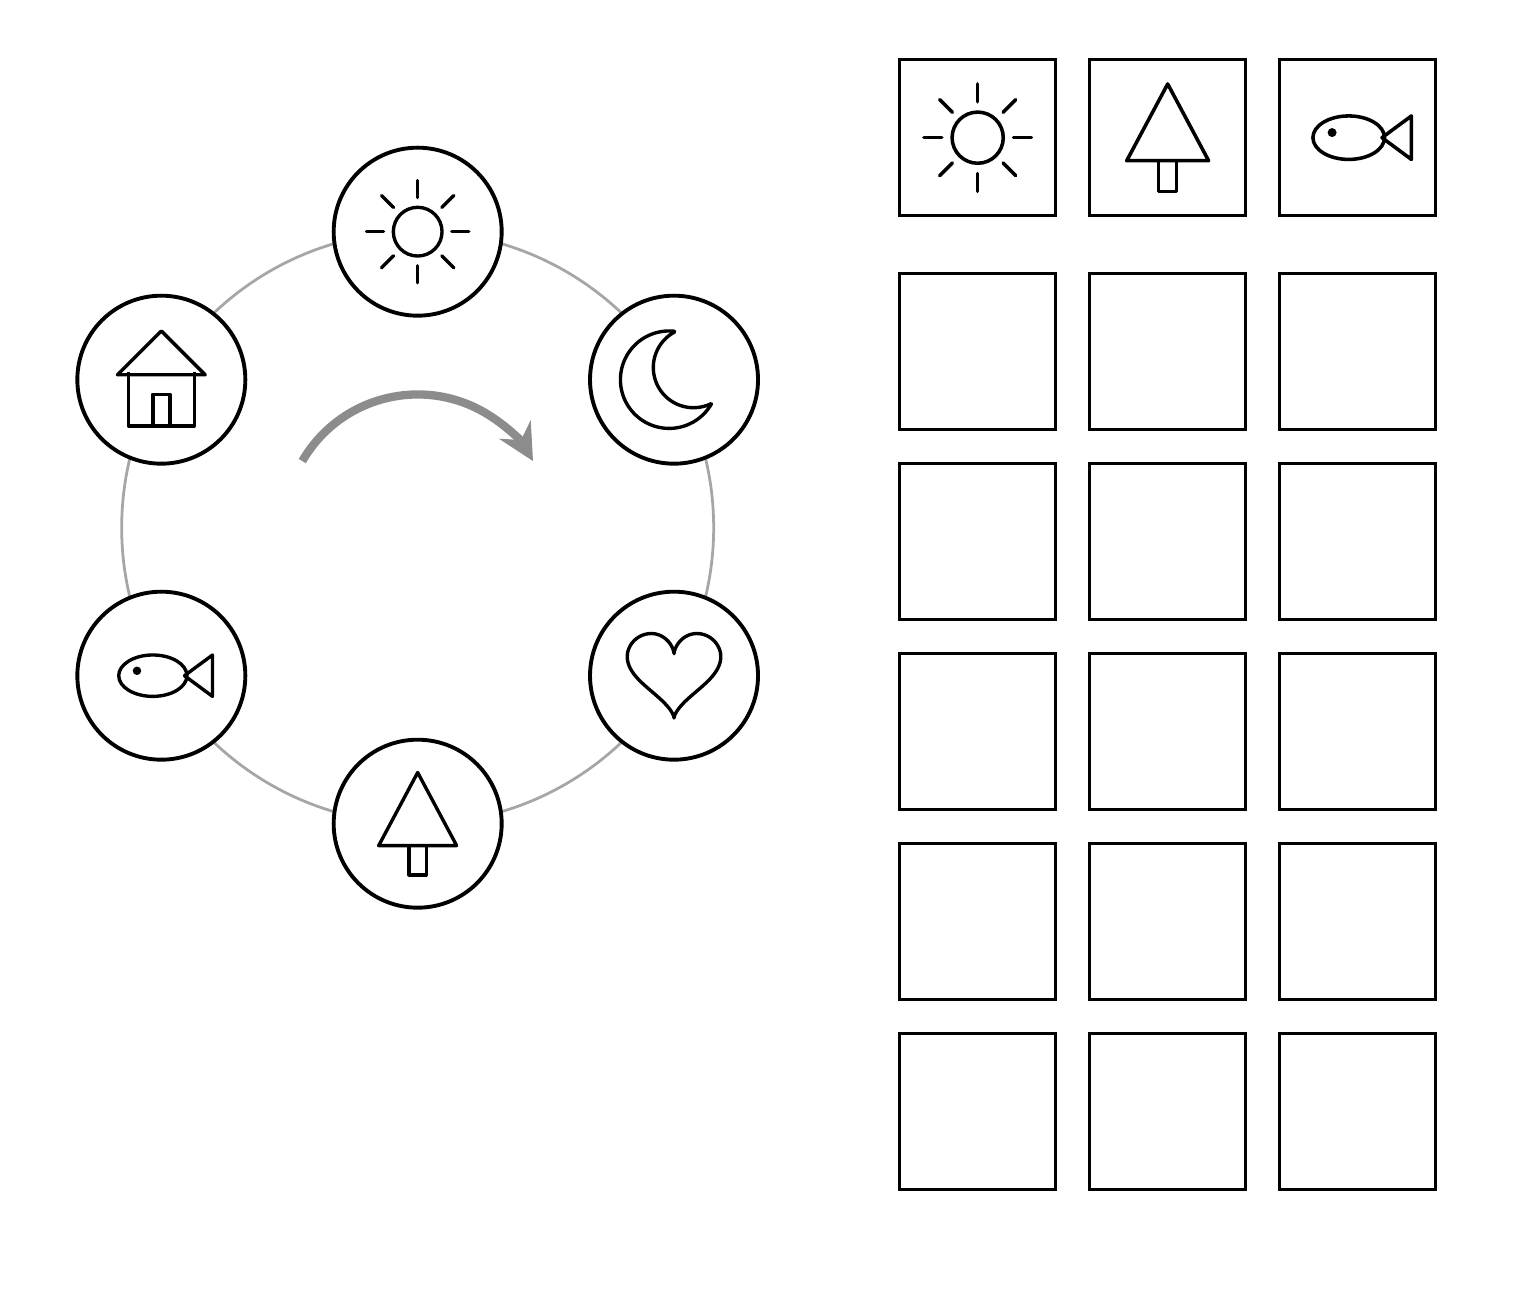
\begin{tikzpicture}[x=1in,y=1in]
\useasboundingbox (0,-6.1) rectangle (7.3,0.1);
\draw[black!35, line width=1pt] (1.95,-2.4) circle (1.48);
\filldraw[fill=white, draw=black, line width=1.4pt] (1.95,-0.92) circle (0.42);
\draw[line width=1.22pt] (1.95,-0.92) circle (0.1218);
\draw[line width=1.22pt, line cap=round] (2.1205,-0.92) -- (2.2058,-0.92);
\draw[line width=1.22pt, line cap=round] (2.0706,-0.7994) -- (2.1309,-0.7391);
\draw[line width=1.22pt, line cap=round] (1.95,-0.7495) -- (1.95,-0.6642);
\draw[line width=1.22pt, line cap=round] (1.8294,-0.7994) -- (1.7691,-0.7391);
\draw[line width=1.22pt, line cap=round] (1.7795,-0.92) -- (1.6942,-0.92);
\draw[line width=1.22pt, line cap=round] (1.8294,-1.0406) -- (1.7691,-1.1009);
\draw[line width=1.22pt, line cap=round] (1.95,-1.0905) -- (1.95,-1.1758);
\draw[line width=1.22pt, line cap=round] (2.0706,-1.0406) -- (2.1309,-1.1009);
\filldraw[fill=white, draw=black, line width=1.4pt] (3.2317,-1.66) circle (0.42);
\draw[line width=1.22pt, line join=round] (3.2328,-1.4177) -- (3.2244,-1.417) -- (3.2159,-1.4165) -- (3.2074,-1.4164) -- (3.1989,-1.4165) -- (3.1904,-1.417) -- (3.1819,-1.4177) -- (3.1735,-1.4188) -- (3.1651,-1.4201) -- (3.1567,-1.4217) -- (3.1484,-1.4236) -- (3.1402,-1.4258) -- (3.1321,-1.4283) -- (3.124,-1.4311) -- (3.1161,-1.4341) -- (3.1083,-1.4375) -- (3.1006,-1.4411) -- (3.093,-1.4449) -- (3.0856,-1.449) -- (3.0783,-1.4534) -- (3.0711,-1.458) -- (3.0642,-1.4629) -- (3.0574,-1.468) -- (3.0508,-1.4734) -- (3.0444,-1.479) -- (3.0381,-1.4848) -- (3.0321,-1.4908) -- (3.0263,-1.497) -- (3.0207,-1.5034) -- (3.0154,-1.51) -- (3.0103,-1.5168) -- (3.0054,-1.5238) -- (3.0008,-1.5309) -- (2.9964,-1.5382) -- (2.9923,-1.5456) -- (2.9884,-1.5532) -- (2.9848,-1.5609) -- (2.9815,-1.5687) -- (2.9784,-1.5767) -- (2.9757,-1.5847) -- (2.9732,-1.5929) -- (2.971,-1.6011) -- (2.9691,-1.6094) -- (2.9675,-1.6177) -- (2.9661,-1.6261) -- (2.9651,-1.6345) -- (2.9644,-1.643) -- (2.9639,-1.6515) -- (2.9638,-1.66) -- (2.9639,-1.6685) -- (2.9644,-1.677) -- (2.9651,-1.6855) -- (2.9661,-1.6939) -- (2.9675,-1.7023) -- (2.9691,-1.7106) -- (2.971,-1.7189) -- (2.9732,-1.7271) -- (2.9757,-1.7353) -- (2.9784,-1.7433) -- (2.9815,-1.7513) -- (2.9848,-1.7591) -- (2.9884,-1.7668) -- (2.9923,-1.7744) -- (2.9964,-1.7818) -- (3.0008,-1.7891) -- (3.0054,-1.7962) -- (3.0103,-1.8032) -- (3.0154,-1.81) -- (3.0207,-1.8166) -- (3.0263,-1.823) -- (3.0321,-1.8292) -- (3.0381,-1.8352) -- (3.0444,-1.841) -- (3.0508,-1.8466) -- (3.0574,-1.852) -- (3.0642,-1.8571) -- (3.0711,-1.862) -- (3.0783,-1.8666) -- (3.0856,-1.871) -- (3.093,-1.8751) -- (3.1006,-1.8789) -- (3.1083,-1.8825) -- (3.1161,-1.8859) -- (3.124,-1.8889) -- (3.1321,-1.8917) -- (3.1402,-1.8942) -- (3.1484,-1.8964) -- (3.1567,-1.8983) -- (3.1651,-1.8999) -- (3.1735,-1.9012) -- (3.1819,-1.9023) -- (3.1904,-1.903) -- (3.1989,-1.9035) -- (3.2074,-1.9036) -- (3.2159,-1.9035) -- (3.2244,-1.903) -- (3.2328,-1.9023) -- (3.2413,-1.9012) -- (3.2497,-1.8999) -- (3.258,-1.8983) -- (3.2663,-1.8964) -- (3.2745,-1.8942) -- (3.2826,-1.8917) -- (3.2907,-1.8889) -- (3.2986,-1.8859) -- (3.3064,-1.8825) -- (3.3141,-1.8789) -- (3.3217,-1.8751) -- (3.3292,-1.871) -- (3.3364,-1.8666) -- (3.3436,-1.862) -- (3.3505,-1.8571) -- (3.3573,-1.852) -- (3.3639,-1.8466) -- (3.3704,-1.841) -- (3.3766,-1.8352) -- (3.3826,-1.8292) -- (3.3884,-1.823) -- (3.394,-1.8166) -- (3.3993,-1.81) -- (3.4044,-1.8032) -- (3.4093,-1.7962) -- (3.4139,-1.7891) -- (3.4183,-1.7818) -- (3.4173,-1.7797) -- (3.4109,-1.7827) -- (3.4044,-1.7854) -- (3.3979,-1.788) -- (3.3913,-1.7902) -- (3.3846,-1.7923) -- (3.3778,-1.7941) -- (3.3709,-1.7957) -- (3.3641,-1.797) -- (3.3571,-1.7981) -- (3.3502,-1.799) -- (3.3432,-1.7996) -- (3.3362,-1.7999) -- (3.3292,-1.8001) -- (3.3221,-1.7999) -- (3.3151,-1.7996) -- (3.3082,-1.799) -- (3.3012,-1.7981) -- (3.2943,-1.797) -- (3.2874,-1.7957) -- (3.2805,-1.7941) -- (3.2738,-1.7923) -- (3.2671,-1.7902) -- (3.2604,-1.788) -- (3.2539,-1.7854) -- (3.2474,-1.7827) -- (3.2411,-1.7797) -- (3.2348,-1.7765) -- (3.2287,-1.7731) -- (3.2227,-1.7695) -- (3.2168,-1.7657) -- (3.211,-1.7617) -- (3.2054,-1.7575) -- (3.2,-1.7531) -- (3.1947,-1.7484) -- (3.1896,-1.7437) -- (3.1846,-1.7387) -- (3.1798,-1.7336) -- (3.1752,-1.7283) -- (3.1708,-1.7228) -- (3.1666,-1.7172) -- (3.1625,-1.7115) -- (3.1587,-1.7056) -- (3.1551,-1.6996) -- (3.1517,-1.6934) -- (3.1485,-1.6872) -- (3.1456,-1.6808) -- (3.1428,-1.6744) -- (3.1403,-1.6678) -- (3.138,-1.6612) -- (3.136,-1.6545) -- (3.1342,-1.6477) -- (3.1326,-1.6409) -- (3.1312,-1.634) -- (3.1301,-1.6271) -- (3.1293,-1.6201) -- (3.1287,-1.6131) -- (3.1283,-1.6061) -- (3.1282,-1.5991) -- (3.1283,-1.5921) -- (3.1287,-1.5851) -- (3.1293,-1.5781) -- (3.1301,-1.5711) -- (3.1312,-1.5642) -- (3.1326,-1.5573) -- (3.1342,-1.5505) -- (3.136,-1.5437) -- (3.138,-1.537) -- (3.1403,-1.5304) -- (3.1428,-1.5238) -- (3.1456,-1.5174) -- (3.1485,-1.511) -- (3.1517,-1.5048) -- (3.1551,-1.4986) -- (3.1587,-1.4926) -- (3.1625,-1.4867) -- (3.1666,-1.481) -- (3.1708,-1.4754) -- (3.1752,-1.4699) -- (3.1798,-1.4646) -- (3.1846,-1.4595) -- (3.1896,-1.4545) -- (3.1947,-1.4498) -- (3.2,-1.4451) -- (3.2054,-1.4407) -- (3.211,-1.4365) -- (3.2168,-1.4325) -- (3.2227,-1.4287) -- (3.2287,-1.4251) -- (3.2348,-1.4217) -- cycle;
\filldraw[fill=white, draw=black, line width=1.4pt] (3.2317,-3.14) circle (0.42);
\draw[line width=1.22pt, line join=round] (3.2317,-3.0304) -- (3.2318,-3.0296) -- (3.232,-3.0271) -- (3.2326,-3.0232) -- (3.2338,-3.0178) -- (3.2358,-3.0112) -- (3.2386,-3.0036) -- (3.2425,-2.9952) -- (3.2475,-2.9863) -- (3.2536,-2.9772) -- (3.2609,-2.9681) -- (3.2695,-2.9595) -- (3.2792,-2.9515) -- (3.29,-2.9444) -- (3.3018,-2.9384) -- (3.3144,-2.9338) -- (3.3277,-2.9307) -- (3.3415,-2.9293) -- (3.3555,-2.9296) -- (3.3697,-2.9316) -- (3.3836,-2.9354) -- (3.3971,-2.9409) -- (3.41,-2.9479) -- (3.422,-2.9565) -- (3.4329,-2.9665) -- (3.4425,-2.9776) -- (3.4506,-2.9898) -- (3.457,-3.0028) -- (3.4618,-3.0164) -- (3.4646,-3.0306) -- (3.4656,-3.045) -- (3.4646,-3.0596) -- (3.4618,-3.0742) -- (3.457,-3.0888) -- (3.4506,-3.1032) -- (3.4425,-3.1173) -- (3.4329,-3.1312) -- (3.422,-3.1448) -- (3.41,-3.1581) -- (3.3971,-3.1711) -- (3.3836,-3.1838) -- (3.3697,-3.1963) -- (3.3555,-3.2085) -- (3.3415,-3.2205) -- (3.3277,-3.2323) -- (3.3144,-3.2439) -- (3.3018,-3.2552) -- (3.29,-3.2662) -- (3.2792,-3.277) -- (3.2695,-3.2873) -- (3.2609,-3.2972) -- (3.2536,-3.3066) -- (3.2475,-3.3154) -- (3.2425,-3.3234) -- (3.2386,-3.3306) -- (3.2358,-3.3369) -- (3.2338,-3.3422) -- (3.2326,-3.3464) -- (3.232,-3.3495) -- (3.2318,-3.3513) -- (3.2317,-3.3519) -- (3.2317,-3.3513) -- (3.2315,-3.3495) -- (3.2308,-3.3464) -- (3.2296,-3.3422) -- (3.2277,-3.3369) -- (3.2248,-3.3306) -- (3.221,-3.3234) -- (3.216,-3.3154) -- (3.2098,-3.3066) -- (3.2025,-3.2972) -- (3.1939,-3.2873) -- (3.1842,-3.277) -- (3.1734,-3.2662) -- (3.1617,-3.2552) -- (3.149,-3.2439) -- (3.1357,-3.2323) -- (3.122,-3.2205) -- (3.1079,-3.2085) -- (3.0938,-3.1963) -- (3.0798,-3.1838) -- (3.0663,-3.1711) -- (3.0534,-3.1581) -- (3.0414,-3.1448) -- (3.0305,-3.1312) -- (3.021,-3.1173) -- (3.0129,-3.1032) -- (3.0064,-3.0888) -- (3.0017,-3.0742) -- (2.9988,-3.0596) -- (2.9979,-3.045) -- (2.9988,-3.0306) -- (3.0017,-3.0164) -- (3.0064,-3.0028) -- (3.0129,-2.9898) -- (3.021,-2.9776) -- (3.0305,-2.9665) -- (3.0414,-2.9565) -- (3.0534,-2.9479) -- (3.0663,-2.9409) -- (3.0798,-2.9354) -- (3.0938,-2.9316) -- (3.1079,-2.9296) -- (3.122,-2.9293) -- (3.1357,-2.9307) -- (3.149,-2.9338) -- (3.1617,-2.9384) -- (3.1734,-2.9444) -- (3.1842,-2.9515) -- (3.1939,-2.9595) -- (3.2025,-2.9681) -- (3.2098,-2.9772) -- (3.216,-2.9863) -- (3.221,-2.9952) -- (3.2248,-3.0036) -- (3.2277,-3.0112) -- (3.2296,-3.0178) -- (3.2308,-3.0232) -- (3.2315,-3.0271) -- (3.2317,-3.0296) -- cycle;
\filldraw[fill=white, draw=black, line width=1.4pt] (1.95,-3.88) circle (0.42);
\draw[line width=1.22pt, line join=round] (1.7551,-3.9896) -- (1.95,-3.6242) -- (2.1449,-3.9896) -- cycle;
\draw[line width=1.22pt, line join=round] (1.9074,-3.9896) -- (1.9074,-4.1358) -- (1.9926,-4.1358) -- (1.9926,-3.9896);
\filldraw[fill=white, draw=black, line width=1.4pt] (0.6683,-3.14) circle (0.42);
\draw[line width=1.22pt] (0.6257,-3.14) ellipse (0.1705 and 0.1035);
\draw[line width=1.22pt, line join=round] (0.784,-3.14) -- (0.9241,-3.0365) -- (0.9241,-3.2435) -- cycle;
\fill (0.5465,-3.1156) circle (0.0213);
\filldraw[fill=white, draw=black, line width=1.4pt] (0.6683,-1.66) circle (0.42);
\draw[line width=1.22pt, line join=round] (0.5039,-1.6235) -- (0.5039,-1.8914) -- (0.8327,-1.8914) -- (0.8327,-1.6235);
\draw[line width=1.22pt, line join=round] (0.449,-1.6356) -- (0.6683,-1.4164) -- (0.8875,-1.6356) -- cycle;
\draw[line width=1.22pt, line join=round] (0.6257,-1.8914) -- (0.6257,-1.7331) -- (0.7109,-1.7331) -- (0.7109,-1.8914);
\draw[black!45, line width=3pt, -{Stealth[length=13pt, width=13pt]}] (1.3732,-2.067) arc[start angle=150, end angle=30, radius=0.666];
\draw[line width=1.2pt] (4.36,-0.84) rectangle (5.14,-0.06);
\draw[line width=1.28pt] (4.75,-0.45) circle (0.1279);
\draw[line width=1.28pt, line cap=round] (4.9291,-0.45) -- (5.0186,-0.45);
\draw[line width=1.28pt, line cap=round] (4.8766,-0.3234) -- (4.94,-0.26);
\draw[line width=1.28pt, line cap=round] (4.75,-0.2709) -- (4.75,-0.1814);
\draw[line width=1.28pt, line cap=round] (4.6234,-0.3234) -- (4.56,-0.26);
\draw[line width=1.28pt, line cap=round] (4.5709,-0.45) -- (4.4814,-0.45);
\draw[line width=1.28pt, line cap=round] (4.6234,-0.5766) -- (4.56,-0.64);
\draw[line width=1.28pt, line cap=round] (4.75,-0.6291) -- (4.75,-0.7186);
\draw[line width=1.28pt, line cap=round] (4.8766,-0.5766) -- (4.94,-0.64);
\draw[line width=1.2pt] (5.31,-0.84) rectangle (6.09,-0.06);
\draw[line width=1.28pt, line join=round] (5.4953,-0.5651) -- (5.7,-0.1814) -- (5.9047,-0.5651) -- cycle;
\draw[line width=1.28pt, line join=round] (5.6552,-0.5651) -- (5.6552,-0.7186) -- (5.7448,-0.7186) -- (5.7448,-0.5651);
\draw[line width=1.2pt] (6.26,-0.84) rectangle (7.04,-0.06);
\draw[line width=1.28pt] (6.6052,-0.45) ellipse (0.1791 and 0.1087);
\draw[line width=1.28pt, line join=round] (6.7715,-0.45) -- (6.9186,-0.3413) -- (6.9186,-0.5587) -- cycle;
\fill (6.5221,-0.4244) circle (0.0224);
\draw[line width=1.2pt] (4.36,-1.91) rectangle (5.14,-1.13);
\draw[line width=1.2pt] (5.31,-1.91) rectangle (6.09,-1.13);
\draw[line width=1.2pt] (6.26,-1.91) rectangle (7.04,-1.13);
\draw[line width=1.2pt] (4.36,-2.86) rectangle (5.14,-2.08);
\draw[line width=1.2pt] (5.31,-2.86) rectangle (6.09,-2.08);
\draw[line width=1.2pt] (6.26,-2.86) rectangle (7.04,-2.08);
\draw[line width=1.2pt] (4.36,-3.81) rectangle (5.14,-3.03);
\draw[line width=1.2pt] (5.31,-3.81) rectangle (6.09,-3.03);
\draw[line width=1.2pt] (6.26,-3.81) rectangle (7.04,-3.03);
\draw[line width=1.2pt] (4.36,-4.76) rectangle (5.14,-3.98);
\draw[line width=1.2pt] (5.31,-4.76) rectangle (6.09,-3.98);
\draw[line width=1.2pt] (6.26,-4.76) rectangle (7.04,-3.98);
\draw[line width=1.2pt] (4.36,-5.71) rectangle (5.14,-4.93);
\draw[line width=1.2pt] (5.31,-5.71) rectangle (6.09,-4.93);
\draw[line width=1.2pt] (6.26,-5.71) rectangle (7.04,-4.93);
\end{tikzpicture}}\par
\vfill

\newpage
\par\vspace{0in}\noindent \prob{9} Which hop changes the picture back to what it was? Write that hop in the box.\par
\par\vspace{0.25in}\noindent\makebox[\textwidth][c]{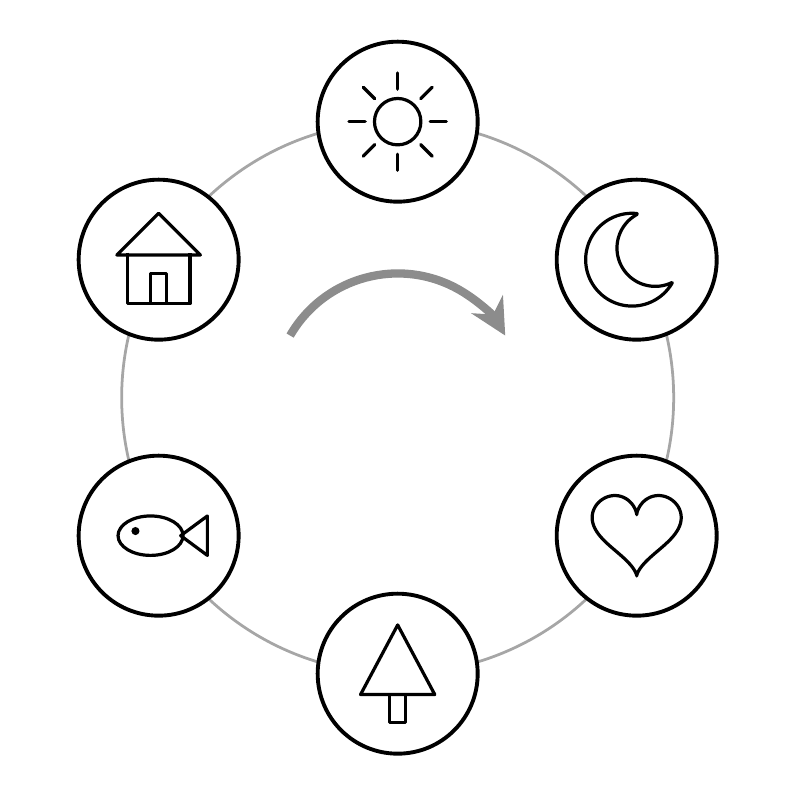
\begin{tikzpicture}[x=1in,y=1in]
\useasboundingbox (-1.85,-1.85) rectangle (1.85,1.85);
\draw[black!35, line width=1pt] (0,0) circle (1.38);
\filldraw[fill=white, draw=black, line width=1.4pt] (0,1.38) circle (0.4);
\draw[line width=1.16pt] (0,1.38) circle (0.116);
\draw[line width=1.16pt, line cap=round] (0.1624,1.38) -- (0.2436,1.38);
\draw[line width=1.16pt, line cap=round] (0.1148,1.4948) -- (0.1723,1.5523);
\draw[line width=1.16pt, line cap=round] (0,1.5424) -- (0,1.6236);
\draw[line width=1.16pt, line cap=round] (-0.1148,1.4948) -- (-0.1723,1.5523);
\draw[line width=1.16pt, line cap=round] (-0.1624,1.38) -- (-0.2436,1.38);
\draw[line width=1.16pt, line cap=round] (-0.1148,1.2652) -- (-0.1723,1.2077);
\draw[line width=1.16pt, line cap=round] (0,1.2176) -- (0,1.1364);
\draw[line width=1.16pt, line cap=round] (0.1148,1.2652) -- (0.1723,1.2077);
\filldraw[fill=white, draw=black, line width=1.4pt] (1.1951,0.69) circle (0.4);
\draw[line width=1.16pt, line join=round] (1.1962,0.9207) -- (1.1881,0.9214) -- (1.18,0.9219) -- (1.1719,0.922) -- (1.1638,0.9219) -- (1.1557,0.9214) -- (1.1477,0.9207) -- (1.1396,0.9197) -- (1.1316,0.9185) -- (1.1237,0.9169) -- (1.1158,0.9151) -- (1.108,0.913) -- (1.1002,0.9106) -- (1.0926,0.908) -- (1.085,0.9051) -- (1.0776,0.9019) -- (1.0702,0.8985) -- (1.063,0.8948) -- (1.0559,0.8909) -- (1.049,0.8867) -- (1.0422,0.8823) -- (1.0355,0.8777) -- (1.0291,0.8728) -- (1.0228,0.8677) -- (1.0167,0.8624) -- (1.0108,0.8569) -- (1.005,0.8512) -- (0.9995,0.8452) -- (0.9942,0.8391) -- (0.9891,0.8328) -- (0.9842,0.8264) -- (0.9796,0.8197) -- (0.9752,0.8129) -- (0.971,0.806) -- (0.9671,0.7989) -- (0.9634,0.7917) -- (0.96,0.7844) -- (0.9568,0.7769) -- (0.9539,0.7693) -- (0.9513,0.7617) -- (0.9489,0.7539) -- (0.9468,0.7461) -- (0.945,0.7382) -- (0.9434,0.7303) -- (0.9422,0.7223) -- (0.9412,0.7143) -- (0.9405,0.7062) -- (0.9401,0.6981) -- (0.9399,0.69) -- (0.9401,0.6819) -- (0.9405,0.6738) -- (0.9412,0.6657) -- (0.9422,0.6577) -- (0.9434,0.6497) -- (0.945,0.6418) -- (0.9468,0.6339) -- (0.9489,0.6261) -- (0.9513,0.6183) -- (0.9539,0.6107) -- (0.9568,0.6031) -- (0.96,0.5956) -- (0.9634,0.5883) -- (0.9671,0.5811) -- (0.971,0.574) -- (0.9752,0.5671) -- (0.9796,0.5603) -- (0.9842,0.5536) -- (0.9891,0.5472) -- (0.9942,0.5409) -- (0.9995,0.5348) -- (1.005,0.5288) -- (1.0108,0.5231) -- (1.0167,0.5176) -- (1.0228,0.5123) -- (1.0291,0.5072) -- (1.0355,0.5023) -- (1.0422,0.4977) -- (1.049,0.4933) -- (1.0559,0.4891) -- (1.063,0.4852) -- (1.0702,0.4815) -- (1.0776,0.4781) -- (1.085,0.4749) -- (1.0926,0.472) -- (1.1002,0.4694) -- (1.108,0.467) -- (1.1158,0.4649) -- (1.1237,0.4631) -- (1.1316,0.4615) -- (1.1396,0.4603) -- (1.1477,0.4593) -- (1.1557,0.4586) -- (1.1638,0.4581) -- (1.1719,0.458) -- (1.18,0.4581) -- (1.1881,0.4586) -- (1.1962,0.4593) -- (1.2042,0.4603) -- (1.2122,0.4615) -- (1.2202,0.4631) -- (1.228,0.4649) -- (1.2359,0.467) -- (1.2436,0.4694) -- (1.2513,0.472) -- (1.2588,0.4749) -- (1.2663,0.4781) -- (1.2736,0.4815) -- (1.2808,0.4852) -- (1.2879,0.4891) -- (1.2949,0.4933) -- (1.3016,0.4977) -- (1.3083,0.5023) -- (1.3147,0.5072) -- (1.321,0.5123) -- (1.3272,0.5176) -- (1.3331,0.5231) -- (1.3388,0.5288) -- (1.3443,0.5348) -- (1.3496,0.5409) -- (1.3547,0.5472) -- (1.3596,0.5536) -- (1.3643,0.5603) -- (1.3687,0.5671) -- (1.3728,0.574) -- (1.3718,0.576) -- (1.3658,0.5731) -- (1.3596,0.5705) -- (1.3534,0.5681) -- (1.3471,0.566) -- (1.3407,0.564) -- (1.3342,0.5623) -- (1.3277,0.5608) -- (1.3212,0.5595) -- (1.3146,0.5585) -- (1.3079,0.5576) -- (1.3013,0.5571) -- (1.2946,0.5567) -- (1.2879,0.5566) -- (1.2812,0.5567) -- (1.2746,0.5571) -- (1.2679,0.5576) -- (1.2613,0.5585) -- (1.2547,0.5595) -- (1.2481,0.5608) -- (1.2416,0.5623) -- (1.2352,0.564) -- (1.2288,0.566) -- (1.2225,0.5681) -- (1.2162,0.5705) -- (1.2101,0.5731) -- (1.204,0.576) -- (1.1981,0.579) -- (1.1922,0.5822) -- (1.1865,0.5857) -- (1.1809,0.5893) -- (1.1754,0.5932) -- (1.1701,0.5972) -- (1.1649,0.6014) -- (1.1598,0.6058) -- (1.155,0.6103) -- (1.1502,0.615) -- (1.1457,0.6199) -- (1.1413,0.625) -- (1.1371,0.6302) -- (1.1331,0.6355) -- (1.1292,0.641) -- (1.1256,0.6466) -- (1.1222,0.6523) -- (1.1189,0.6581) -- (1.1159,0.6641) -- (1.1131,0.6702) -- (1.1105,0.6763) -- (1.1081,0.6825) -- (1.1059,0.6889) -- (1.1039,0.6952) -- (1.1022,0.7017) -- (1.1007,0.7082) -- (1.0994,0.7148) -- (1.0984,0.7214) -- (1.0976,0.728) -- (1.097,0.7346) -- (1.0966,0.7413) -- (1.0965,0.748) -- (1.0966,0.7547) -- (1.097,0.7614) -- (1.0976,0.768) -- (1.0984,0.7746) -- (1.0994,0.7812) -- (1.1007,0.7878) -- (1.1022,0.7943) -- (1.1039,0.8008) -- (1.1059,0.8071) -- (1.1081,0.8135) -- (1.1105,0.8197) -- (1.1131,0.8258) -- (1.1159,0.8319) -- (1.1189,0.8379) -- (1.1222,0.8437) -- (1.1256,0.8494) -- (1.1292,0.855) -- (1.1331,0.8605) -- (1.1371,0.8658) -- (1.1413,0.871) -- (1.1457,0.8761) -- (1.1502,0.881) -- (1.155,0.8857) -- (1.1598,0.8902) -- (1.1649,0.8946) -- (1.1701,0.8988) -- (1.1754,0.9028) -- (1.1809,0.9067) -- (1.1865,0.9103) -- (1.1922,0.9138) -- (1.1981,0.917) -- cycle;
\filldraw[fill=white, draw=black, line width=1.4pt] (1.1951,-0.69) circle (0.4);
\draw[line width=1.16pt, line join=round] (1.1951,-0.5856) -- (1.1951,-0.5848) -- (1.1954,-0.5825) -- (1.196,-0.5787) -- (1.1971,-0.5736) -- (1.199,-0.5673) -- (1.2017,-0.5601) -- (1.2054,-0.5521) -- (1.2101,-0.5436) -- (1.216,-0.5349) -- (1.223,-0.5263) -- (1.2311,-0.5181) -- (1.2403,-0.5104) -- (1.2506,-0.5037) -- (1.2618,-0.498) -- (1.2739,-0.4936) -- (1.2865,-0.4907) -- (1.2997,-0.4893) -- (1.313,-0.4896) -- (1.3265,-0.4915) -- (1.3398,-0.4951) -- (1.3527,-0.5003) -- (1.3649,-0.5071) -- (1.3763,-0.5153) -- (1.3867,-0.5248) -- (1.3958,-0.5354) -- (1.4036,-0.5469) -- (1.4097,-0.5593) -- (1.4142,-0.5723) -- (1.4169,-0.5858) -- (1.4178,-0.5995) -- (1.4169,-0.6134) -- (1.4142,-0.6274) -- (1.4097,-0.6412) -- (1.4036,-0.6549) -- (1.3958,-0.6684) -- (1.3867,-0.6816) -- (1.3763,-0.6946) -- (1.3649,-0.7073) -- (1.3527,-0.7196) -- (1.3398,-0.7318) -- (1.3265,-0.7436) -- (1.313,-0.7553) -- (1.2997,-0.7667) -- (1.2865,-0.7779) -- (1.2739,-0.7889) -- (1.2618,-0.7997) -- (1.2506,-0.8102) -- (1.2403,-0.8204) -- (1.2311,-0.8303) -- (1.223,-0.8398) -- (1.216,-0.8487) -- (1.2101,-0.857) -- (1.2054,-0.8647) -- (1.2017,-0.8715) -- (1.199,-0.8775) -- (1.1971,-0.8826) -- (1.196,-0.8866) -- (1.1954,-0.8895) -- (1.1951,-0.8912) -- (1.1951,-0.8918) -- (1.1951,-0.8912) -- (1.1949,-0.8895) -- (1.1943,-0.8866) -- (1.1931,-0.8826) -- (1.1913,-0.8775) -- (1.1885,-0.8715) -- (1.1849,-0.8647) -- (1.1801,-0.857) -- (1.1743,-0.8487) -- (1.1673,-0.8398) -- (1.1591,-0.8303) -- (1.1499,-0.8204) -- (1.1396,-0.8102) -- (1.1284,-0.7997) -- (1.1164,-0.7889) -- (1.1037,-0.7779) -- (1.0906,-0.7667) -- (1.0772,-0.7553) -- (1.0637,-0.7436) -- (1.0505,-0.7318) -- (1.0376,-0.7196) -- (1.0253,-0.7073) -- (1.0139,-0.6946) -- (1.0035,-0.6816) -- (0.9944,-0.6684) -- (0.9867,-0.6549) -- (0.9805,-0.6412) -- (0.976,-0.6274) -- (0.9733,-0.6134) -- (0.9724,-0.5995) -- (0.9733,-0.5858) -- (0.976,-0.5723) -- (0.9805,-0.5593) -- (0.9867,-0.5469) -- (0.9944,-0.5354) -- (1.0035,-0.5248) -- (1.0139,-0.5153) -- (1.0253,-0.5071) -- (1.0376,-0.5003) -- (1.0505,-0.4951) -- (1.0637,-0.4915) -- (1.0772,-0.4896) -- (1.0906,-0.4893) -- (1.1037,-0.4907) -- (1.1164,-0.4936) -- (1.1284,-0.498) -- (1.1396,-0.5037) -- (1.1499,-0.5104) -- (1.1591,-0.5181) -- (1.1673,-0.5263) -- (1.1743,-0.5349) -- (1.1801,-0.5436) -- (1.1849,-0.5521) -- (1.1885,-0.5601) -- (1.1913,-0.5673) -- (1.1931,-0.5736) -- (1.1943,-0.5787) -- (1.1949,-0.5825) -- (1.1951,-0.5848) -- cycle;
\filldraw[fill=white, draw=black, line width=1.4pt] (0,-1.38) circle (0.4);
\draw[line width=1.16pt, line join=round] (-0.1856,-1.4844) -- (0,-1.1364) -- (0.1856,-1.4844) -- cycle;
\draw[line width=1.16pt, line join=round] (-0.0406,-1.4844) -- (-0.0406,-1.6236) -- (0.0406,-1.6236) -- (0.0406,-1.4844);
\filldraw[fill=white, draw=black, line width=1.4pt] (-1.1951,-0.69) circle (0.4);
\draw[line width=1.16pt] (-1.2357,-0.69) ellipse (0.1624 and 0.0986);
\draw[line width=1.16pt, line join=round] (-1.0849,-0.69) -- (-0.9515,-0.5914) -- (-0.9515,-0.7886) -- cycle;
\fill (-1.3111,-0.6668) circle (0.0203);
\filldraw[fill=white, draw=black, line width=1.4pt] (-1.1951,0.69) circle (0.4);
\draw[line width=1.16pt, line join=round] (-1.3517,0.7248) -- (-1.3517,0.4696) -- (-1.0385,0.4696) -- (-1.0385,0.7248);
\draw[line width=1.16pt, line join=round] (-1.4039,0.7132) -- (-1.1951,0.922) -- (-0.9863,0.7132) -- cycle;
\draw[line width=1.16pt, line join=round] (-1.2357,0.4696) -- (-1.2357,0.6204) -- (-1.1545,0.6204) -- (-1.1545,0.4696);
\draw[black!45, line width=3pt, -{Stealth[length=13pt, width=13pt]}] (-0.5378,0.3105) arc[start angle=150, end angle=30, radius=0.621];
\end{tikzpicture}}\par
\par\vspace{0.35in}\noindent\makebox[\textwidth][c]{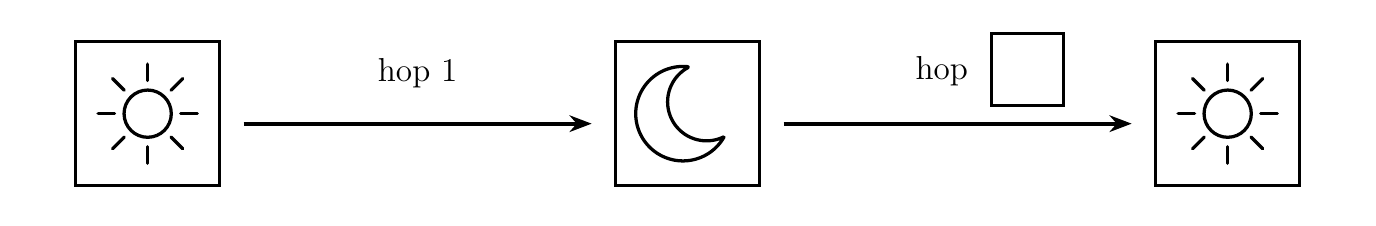
\begin{tikzpicture}[x=1in,y=1in]
\useasboundingbox (0,-0.42) rectangle (6.6,0.43);
\draw[line width=1.2pt] (0.24,-0.36) rectangle (0.96,0.36);
\draw[line width=1.18pt] (0.6,0) circle (0.1181);
\draw[line width=1.18pt, line cap=round] (0.7653,0) -- (0.848,0);
\draw[line width=1.18pt, line cap=round] (0.7169,0.1169) -- (0.7753,0.1753);
\draw[line width=1.18pt, line cap=round] (0.6,0.1653) -- (0.6,0.248);
\draw[line width=1.18pt, line cap=round] (0.4831,0.1169) -- (0.4247,0.1753);
\draw[line width=1.18pt, line cap=round] (0.4347,0) -- (0.352,0);
\draw[line width=1.18pt, line cap=round] (0.4831,-0.1169) -- (0.4247,-0.1753);
\draw[line width=1.18pt, line cap=round] (0.6,-0.1653) -- (0.6,-0.248);
\draw[line width=1.18pt, line cap=round] (0.7169,-0.1169) -- (0.7753,-0.1753);
\draw[line width=1.2pt] (2.94,-0.36) rectangle (3.66,0.36);
\draw[line width=1.18pt, line join=round] (3.3011,0.2349) -- (3.2929,0.2356) -- (3.2846,0.236) -- (3.2764,0.2362) -- (3.2681,0.236) -- (3.2599,0.2356) -- (3.2517,0.2349) -- (3.2435,0.2339) -- (3.2354,0.2326) -- (3.2273,0.231) -- (3.2193,0.2291) -- (3.2113,0.227) -- (3.2034,0.2246) -- (3.1956,0.2219) -- (3.1879,0.219) -- (3.1803,0.2157) -- (3.1729,0.2123) -- (3.1655,0.2085) -- (3.1583,0.2045) -- (3.1512,0.2003) -- (3.1443,0.1958) -- (3.1376,0.1911) -- (3.131,0.1861) -- (3.1246,0.1809) -- (3.1184,0.1755) -- (3.1123,0.1699) -- (3.1065,0.1641) -- (3.1009,0.158) -- (3.0955,0.1518) -- (3.0903,0.1454) -- (3.0853,0.1388) -- (3.0806,0.1321) -- (3.0761,0.1251) -- (3.0719,0.1181) -- (3.0679,0.1109) -- (3.0641,0.1035) -- (3.0606,0.0961) -- (3.0574,0.0885) -- (3.0545,0.0808) -- (3.0518,0.073) -- (3.0494,0.0651) -- (3.0472,0.0571) -- (3.0454,0.0491) -- (3.0438,0.041) -- (3.0425,0.0329) -- (3.0415,0.0247) -- (3.0408,0.0165) -- (3.0404,0.0082) -- (3.0402,0) -- (3.0404,-0.0082) -- (3.0408,-0.0165) -- (3.0415,-0.0247) -- (3.0425,-0.0329) -- (3.0438,-0.041) -- (3.0454,-0.0491) -- (3.0472,-0.0571) -- (3.0494,-0.0651) -- (3.0518,-0.073) -- (3.0545,-0.0808) -- (3.0574,-0.0885) -- (3.0606,-0.0961) -- (3.0641,-0.1035) -- (3.0679,-0.1109) -- (3.0719,-0.1181) -- (3.0761,-0.1251) -- (3.0806,-0.1321) -- (3.0853,-0.1388) -- (3.0903,-0.1454) -- (3.0955,-0.1518) -- (3.1009,-0.158) -- (3.1065,-0.1641) -- (3.1123,-0.1699) -- (3.1184,-0.1755) -- (3.1246,-0.1809) -- (3.131,-0.1861) -- (3.1376,-0.1911) -- (3.1443,-0.1958) -- (3.1512,-0.2003) -- (3.1583,-0.2045) -- (3.1655,-0.2085) -- (3.1729,-0.2123) -- (3.1803,-0.2157) -- (3.1879,-0.219) -- (3.1956,-0.2219) -- (3.2034,-0.2246) -- (3.2113,-0.227) -- (3.2193,-0.2291) -- (3.2273,-0.231) -- (3.2354,-0.2326) -- (3.2435,-0.2339) -- (3.2517,-0.2349) -- (3.2599,-0.2356) -- (3.2681,-0.236) -- (3.2764,-0.2362) -- (3.2846,-0.236) -- (3.2929,-0.2356) -- (3.3011,-0.2349) -- (3.3093,-0.2339) -- (3.3174,-0.2326) -- (3.3255,-0.231) -- (3.3335,-0.2291) -- (3.3415,-0.227) -- (3.3494,-0.2246) -- (3.3572,-0.2219) -- (3.3649,-0.219) -- (3.3724,-0.2157) -- (3.3799,-0.2123) -- (3.3873,-0.2085) -- (3.3945,-0.2045) -- (3.4015,-0.2003) -- (3.4084,-0.1958) -- (3.4152,-0.1911) -- (3.4218,-0.1861) -- (3.4282,-0.1809) -- (3.4344,-0.1755) -- (3.4404,-0.1699) -- (3.4463,-0.1641) -- (3.4519,-0.158) -- (3.4573,-0.1518) -- (3.4625,-0.1454) -- (3.4674,-0.1388) -- (3.4722,-0.1321) -- (3.4767,-0.1251) -- (3.4809,-0.1181) -- (3.4799,-0.1161) -- (3.4737,-0.1189) -- (3.4674,-0.1216) -- (3.4611,-0.124) -- (3.4547,-0.1263) -- (3.4482,-0.1282) -- (3.4416,-0.13) -- (3.435,-0.1315) -- (3.4283,-0.1328) -- (3.4216,-0.1339) -- (3.4148,-0.1347) -- (3.4081,-0.1353) -- (3.4013,-0.1357) -- (3.3945,-0.1358) -- (3.3877,-0.1357) -- (3.3809,-0.1353) -- (3.3741,-0.1347) -- (3.3673,-0.1339) -- (3.3606,-0.1328) -- (3.354,-0.1315) -- (3.3473,-0.13) -- (3.3408,-0.1282) -- (3.3343,-0.1263) -- (3.3278,-0.124) -- (3.3215,-0.1216) -- (3.3152,-0.1189) -- (3.3091,-0.1161) -- (3.303,-0.113) -- (3.297,-0.1097) -- (3.2912,-0.1062) -- (3.2855,-0.1025) -- (3.2799,-0.0986) -- (3.2745,-0.0945) -- (3.2692,-0.0902) -- (3.2641,-0.0857) -- (3.2591,-0.0811) -- (3.2543,-0.0763) -- (3.2497,-0.0713) -- (3.2452,-0.0662) -- (3.2409,-0.0609) -- (3.2368,-0.0555) -- (3.2329,-0.0499) -- (3.2292,-0.0442) -- (3.2257,-0.0384) -- (3.2224,-0.0324) -- (3.2194,-0.0264) -- (3.2165,-0.0202) -- (3.2138,-0.0139) -- (3.2114,-0.0076) -- (3.2092,-0.0012) -- (3.2072,0.0053) -- (3.2054,0.0119) -- (3.2039,0.0185) -- (3.2026,0.0252) -- (3.2015,0.0319) -- (3.2007,0.0387) -- (3.2001,0.0454) -- (3.1998,0.0522) -- (3.1996,0.059) -- (3.1998,0.0658) -- (3.2001,0.0726) -- (3.2007,0.0794) -- (3.2015,0.0862) -- (3.2026,0.0929) -- (3.2039,0.0995) -- (3.2054,0.1062) -- (3.2072,0.1127) -- (3.2092,0.1192) -- (3.2114,0.1257) -- (3.2138,0.132) -- (3.2165,0.1383) -- (3.2194,0.1444) -- (3.2224,0.1505) -- (3.2257,0.1565) -- (3.2292,0.1623) -- (3.2329,0.168) -- (3.2368,0.1736) -- (3.2409,0.179) -- (3.2452,0.1843) -- (3.2497,0.1894) -- (3.2543,0.1944) -- (3.2591,0.1992) -- (3.2641,0.2038) -- (3.2692,0.2083) -- (3.2745,0.2126) -- (3.2799,0.2167) -- (3.2855,0.2206) -- (3.2912,0.2243) -- (3.297,0.2278) -- (3.303,0.2311) -- cycle;
\draw[line width=1.2pt] (5.64,-0.36) rectangle (6.36,0.36);
\draw[line width=1.18pt] (6,0) circle (0.1181);
\draw[line width=1.18pt, line cap=round] (6.1653,0) -- (6.248,0);
\draw[line width=1.18pt, line cap=round] (6.1169,0.1169) -- (6.1753,0.1753);
\draw[line width=1.18pt, line cap=round] (6,0.1653) -- (6,0.248);
\draw[line width=1.18pt, line cap=round] (5.8831,0.1169) -- (5.8247,0.1753);
\draw[line width=1.18pt, line cap=round] (5.8347,0) -- (5.752,0);
\draw[line width=1.18pt, line cap=round] (5.8831,-0.1169) -- (5.8247,-0.1753);
\draw[line width=1.18pt, line cap=round] (6,-0.1653) -- (6,-0.248);
\draw[line width=1.18pt, line cap=round] (6.1169,-0.1169) -- (6.1753,-0.1753);
\draw[line width=1.4pt, -{Stealth[length=8pt]}] (1.08,-0.05) -- (2.82,-0.05);
\node[font=\large] at (1.95,0.2) {hop 1};
\draw[line width=1.4pt, -{Stealth[length=8pt]}] (3.78,-0.05) -- (5.52,-0.05);
\node[font=\large, anchor=east] at (4.75,0.21) {hop};
\draw[line width=1pt] (4.82,0.04) rectangle (5.18,0.4);
\end{tikzpicture}}\par
\par\vspace{0.18in}\noindent\makebox[\textwidth][c]{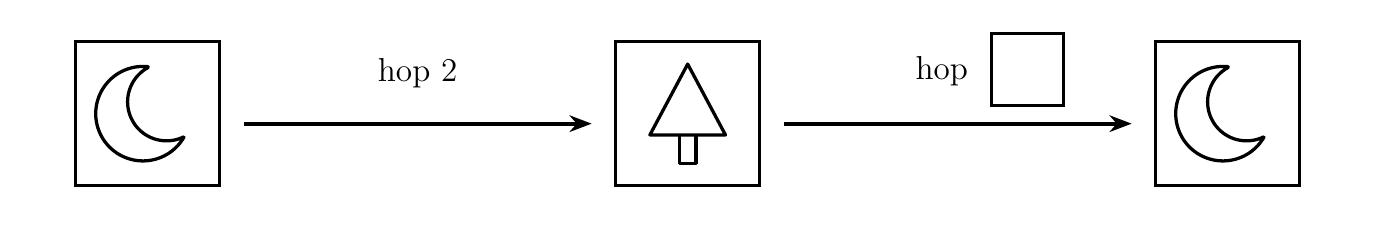
\begin{tikzpicture}[x=1in,y=1in]
\useasboundingbox (0,-0.42) rectangle (6.6,0.43);
\draw[line width=1.2pt] (0.24,-0.36) rectangle (0.96,0.36);
\draw[line width=1.18pt, line join=round] (0.6011,0.2349) -- (0.5929,0.2356) -- (0.5846,0.236) -- (0.5764,0.2362) -- (0.5681,0.236) -- (0.5599,0.2356) -- (0.5517,0.2349) -- (0.5435,0.2339) -- (0.5354,0.2326) -- (0.5273,0.231) -- (0.5193,0.2291) -- (0.5113,0.227) -- (0.5034,0.2246) -- (0.4956,0.2219) -- (0.4879,0.219) -- (0.4803,0.2157) -- (0.4729,0.2123) -- (0.4655,0.2085) -- (0.4583,0.2045) -- (0.4512,0.2003) -- (0.4443,0.1958) -- (0.4376,0.1911) -- (0.431,0.1861) -- (0.4246,0.1809) -- (0.4184,0.1755) -- (0.4123,0.1699) -- (0.4065,0.1641) -- (0.4009,0.158) -- (0.3955,0.1518) -- (0.3903,0.1454) -- (0.3853,0.1388) -- (0.3806,0.1321) -- (0.3761,0.1251) -- (0.3719,0.1181) -- (0.3679,0.1109) -- (0.3641,0.1035) -- (0.3606,0.0961) -- (0.3574,0.0885) -- (0.3545,0.0808) -- (0.3518,0.073) -- (0.3494,0.0651) -- (0.3472,0.0571) -- (0.3454,0.0491) -- (0.3438,0.041) -- (0.3425,0.0329) -- (0.3415,0.0247) -- (0.3408,0.0165) -- (0.3404,0.0082) -- (0.3402,0) -- (0.3404,-0.0082) -- (0.3408,-0.0165) -- (0.3415,-0.0247) -- (0.3425,-0.0329) -- (0.3438,-0.041) -- (0.3454,-0.0491) -- (0.3472,-0.0571) -- (0.3494,-0.0651) -- (0.3518,-0.073) -- (0.3545,-0.0808) -- (0.3574,-0.0885) -- (0.3606,-0.0961) -- (0.3641,-0.1035) -- (0.3679,-0.1109) -- (0.3719,-0.1181) -- (0.3761,-0.1251) -- (0.3806,-0.1321) -- (0.3853,-0.1388) -- (0.3903,-0.1454) -- (0.3955,-0.1518) -- (0.4009,-0.158) -- (0.4065,-0.1641) -- (0.4123,-0.1699) -- (0.4184,-0.1755) -- (0.4246,-0.1809) -- (0.431,-0.1861) -- (0.4376,-0.1911) -- (0.4443,-0.1958) -- (0.4512,-0.2003) -- (0.4583,-0.2045) -- (0.4655,-0.2085) -- (0.4729,-0.2123) -- (0.4803,-0.2157) -- (0.4879,-0.219) -- (0.4956,-0.2219) -- (0.5034,-0.2246) -- (0.5113,-0.227) -- (0.5193,-0.2291) -- (0.5273,-0.231) -- (0.5354,-0.2326) -- (0.5435,-0.2339) -- (0.5517,-0.2349) -- (0.5599,-0.2356) -- (0.5681,-0.236) -- (0.5764,-0.2362) -- (0.5846,-0.236) -- (0.5929,-0.2356) -- (0.6011,-0.2349) -- (0.6093,-0.2339) -- (0.6174,-0.2326) -- (0.6255,-0.231) -- (0.6335,-0.2291) -- (0.6415,-0.227) -- (0.6494,-0.2246) -- (0.6572,-0.2219) -- (0.6649,-0.219) -- (0.6724,-0.2157) -- (0.6799,-0.2123) -- (0.6873,-0.2085) -- (0.6945,-0.2045) -- (0.7015,-0.2003) -- (0.7084,-0.1958) -- (0.7152,-0.1911) -- (0.7218,-0.1861) -- (0.7282,-0.1809) -- (0.7344,-0.1755) -- (0.7404,-0.1699) -- (0.7463,-0.1641) -- (0.7519,-0.158) -- (0.7573,-0.1518) -- (0.7625,-0.1454) -- (0.7674,-0.1388) -- (0.7722,-0.1321) -- (0.7767,-0.1251) -- (0.7809,-0.1181) -- (0.7799,-0.1161) -- (0.7737,-0.1189) -- (0.7674,-0.1216) -- (0.7611,-0.124) -- (0.7547,-0.1263) -- (0.7482,-0.1282) -- (0.7416,-0.13) -- (0.735,-0.1315) -- (0.7283,-0.1328) -- (0.7216,-0.1339) -- (0.7148,-0.1347) -- (0.7081,-0.1353) -- (0.7013,-0.1357) -- (0.6945,-0.1358) -- (0.6877,-0.1357) -- (0.6809,-0.1353) -- (0.6741,-0.1347) -- (0.6673,-0.1339) -- (0.6606,-0.1328) -- (0.654,-0.1315) -- (0.6473,-0.13) -- (0.6408,-0.1282) -- (0.6343,-0.1263) -- (0.6278,-0.124) -- (0.6215,-0.1216) -- (0.6152,-0.1189) -- (0.6091,-0.1161) -- (0.603,-0.113) -- (0.597,-0.1097) -- (0.5912,-0.1062) -- (0.5855,-0.1025) -- (0.5799,-0.0986) -- (0.5745,-0.0945) -- (0.5692,-0.0902) -- (0.5641,-0.0857) -- (0.5591,-0.0811) -- (0.5543,-0.0763) -- (0.5497,-0.0713) -- (0.5452,-0.0662) -- (0.5409,-0.0609) -- (0.5368,-0.0555) -- (0.5329,-0.0499) -- (0.5292,-0.0442) -- (0.5257,-0.0384) -- (0.5224,-0.0324) -- (0.5194,-0.0264) -- (0.5165,-0.0202) -- (0.5138,-0.0139) -- (0.5114,-0.0076) -- (0.5092,-0.0012) -- (0.5072,0.0053) -- (0.5054,0.0119) -- (0.5039,0.0185) -- (0.5026,0.0252) -- (0.5015,0.0319) -- (0.5007,0.0387) -- (0.5001,0.0454) -- (0.4998,0.0522) -- (0.4996,0.059) -- (0.4998,0.0658) -- (0.5001,0.0726) -- (0.5007,0.0794) -- (0.5015,0.0862) -- (0.5026,0.0929) -- (0.5039,0.0995) -- (0.5054,0.1062) -- (0.5072,0.1127) -- (0.5092,0.1192) -- (0.5114,0.1257) -- (0.5138,0.132) -- (0.5165,0.1383) -- (0.5194,0.1444) -- (0.5224,0.1505) -- (0.5257,0.1565) -- (0.5292,0.1623) -- (0.5329,0.168) -- (0.5368,0.1736) -- (0.5409,0.179) -- (0.5452,0.1843) -- (0.5497,0.1894) -- (0.5543,0.1944) -- (0.5591,0.1992) -- (0.5641,0.2038) -- (0.5692,0.2083) -- (0.5745,0.2126) -- (0.5799,0.2167) -- (0.5855,0.2206) -- (0.5912,0.2243) -- (0.597,0.2278) -- (0.603,0.2311) -- cycle;
\draw[line width=1.2pt] (2.94,-0.36) rectangle (3.66,0.36);
\draw[line width=1.18pt, line join=round] (3.1111,-0.1063) -- (3.3,0.248) -- (3.4889,-0.1063) -- cycle;
\draw[line width=1.18pt, line join=round] (3.2587,-0.1063) -- (3.2587,-0.248) -- (3.3413,-0.248) -- (3.3413,-0.1063);
\draw[line width=1.2pt] (5.64,-0.36) rectangle (6.36,0.36);
\draw[line width=1.18pt, line join=round] (6.0011,0.2349) -- (5.9929,0.2356) -- (5.9846,0.236) -- (5.9764,0.2362) -- (5.9681,0.236) -- (5.9599,0.2356) -- (5.9517,0.2349) -- (5.9435,0.2339) -- (5.9354,0.2326) -- (5.9273,0.231) -- (5.9193,0.2291) -- (5.9113,0.227) -- (5.9034,0.2246) -- (5.8956,0.2219) -- (5.8879,0.219) -- (5.8803,0.2157) -- (5.8729,0.2123) -- (5.8655,0.2085) -- (5.8583,0.2045) -- (5.8512,0.2003) -- (5.8443,0.1958) -- (5.8376,0.1911) -- (5.831,0.1861) -- (5.8246,0.1809) -- (5.8184,0.1755) -- (5.8123,0.1699) -- (5.8065,0.1641) -- (5.8009,0.158) -- (5.7955,0.1518) -- (5.7903,0.1454) -- (5.7853,0.1388) -- (5.7806,0.1321) -- (5.7761,0.1251) -- (5.7719,0.1181) -- (5.7679,0.1109) -- (5.7641,0.1035) -- (5.7606,0.0961) -- (5.7574,0.0885) -- (5.7545,0.0808) -- (5.7518,0.073) -- (5.7494,0.0651) -- (5.7472,0.0571) -- (5.7454,0.0491) -- (5.7438,0.041) -- (5.7425,0.0329) -- (5.7415,0.0247) -- (5.7408,0.0165) -- (5.7404,0.0082) -- (5.7402,0) -- (5.7404,-0.0082) -- (5.7408,-0.0165) -- (5.7415,-0.0247) -- (5.7425,-0.0329) -- (5.7438,-0.041) -- (5.7454,-0.0491) -- (5.7472,-0.0571) -- (5.7494,-0.0651) -- (5.7518,-0.073) -- (5.7545,-0.0808) -- (5.7574,-0.0885) -- (5.7606,-0.0961) -- (5.7641,-0.1035) -- (5.7679,-0.1109) -- (5.7719,-0.1181) -- (5.7761,-0.1251) -- (5.7806,-0.1321) -- (5.7853,-0.1388) -- (5.7903,-0.1454) -- (5.7955,-0.1518) -- (5.8009,-0.158) -- (5.8065,-0.1641) -- (5.8123,-0.1699) -- (5.8184,-0.1755) -- (5.8246,-0.1809) -- (5.831,-0.1861) -- (5.8376,-0.1911) -- (5.8443,-0.1958) -- (5.8512,-0.2003) -- (5.8583,-0.2045) -- (5.8655,-0.2085) -- (5.8729,-0.2123) -- (5.8803,-0.2157) -- (5.8879,-0.219) -- (5.8956,-0.2219) -- (5.9034,-0.2246) -- (5.9113,-0.227) -- (5.9193,-0.2291) -- (5.9273,-0.231) -- (5.9354,-0.2326) -- (5.9435,-0.2339) -- (5.9517,-0.2349) -- (5.9599,-0.2356) -- (5.9681,-0.236) -- (5.9764,-0.2362) -- (5.9846,-0.236) -- (5.9929,-0.2356) -- (6.0011,-0.2349) -- (6.0093,-0.2339) -- (6.0174,-0.2326) -- (6.0255,-0.231) -- (6.0335,-0.2291) -- (6.0415,-0.227) -- (6.0494,-0.2246) -- (6.0572,-0.2219) -- (6.0649,-0.219) -- (6.0724,-0.2157) -- (6.0799,-0.2123) -- (6.0873,-0.2085) -- (6.0945,-0.2045) -- (6.1015,-0.2003) -- (6.1084,-0.1958) -- (6.1152,-0.1911) -- (6.1218,-0.1861) -- (6.1282,-0.1809) -- (6.1344,-0.1755) -- (6.1404,-0.1699) -- (6.1463,-0.1641) -- (6.1519,-0.158) -- (6.1573,-0.1518) -- (6.1625,-0.1454) -- (6.1674,-0.1388) -- (6.1722,-0.1321) -- (6.1767,-0.1251) -- (6.1809,-0.1181) -- (6.1799,-0.1161) -- (6.1737,-0.1189) -- (6.1674,-0.1216) -- (6.1611,-0.124) -- (6.1547,-0.1263) -- (6.1482,-0.1282) -- (6.1416,-0.13) -- (6.135,-0.1315) -- (6.1283,-0.1328) -- (6.1216,-0.1339) -- (6.1148,-0.1347) -- (6.1081,-0.1353) -- (6.1013,-0.1357) -- (6.0945,-0.1358) -- (6.0877,-0.1357) -- (6.0809,-0.1353) -- (6.0741,-0.1347) -- (6.0673,-0.1339) -- (6.0606,-0.1328) -- (6.054,-0.1315) -- (6.0473,-0.13) -- (6.0408,-0.1282) -- (6.0343,-0.1263) -- (6.0278,-0.124) -- (6.0215,-0.1216) -- (6.0152,-0.1189) -- (6.0091,-0.1161) -- (6.003,-0.113) -- (5.997,-0.1097) -- (5.9912,-0.1062) -- (5.9855,-0.1025) -- (5.9799,-0.0986) -- (5.9745,-0.0945) -- (5.9692,-0.0902) -- (5.9641,-0.0857) -- (5.9591,-0.0811) -- (5.9543,-0.0763) -- (5.9497,-0.0713) -- (5.9452,-0.0662) -- (5.9409,-0.0609) -- (5.9368,-0.0555) -- (5.9329,-0.0499) -- (5.9292,-0.0442) -- (5.9257,-0.0384) -- (5.9224,-0.0324) -- (5.9194,-0.0264) -- (5.9165,-0.0202) -- (5.9138,-0.0139) -- (5.9114,-0.0076) -- (5.9092,-0.0012) -- (5.9072,0.0053) -- (5.9054,0.0119) -- (5.9039,0.0185) -- (5.9026,0.0252) -- (5.9015,0.0319) -- (5.9007,0.0387) -- (5.9001,0.0454) -- (5.8998,0.0522) -- (5.8996,0.059) -- (5.8998,0.0658) -- (5.9001,0.0726) -- (5.9007,0.0794) -- (5.9015,0.0862) -- (5.9026,0.0929) -- (5.9039,0.0995) -- (5.9054,0.1062) -- (5.9072,0.1127) -- (5.9092,0.1192) -- (5.9114,0.1257) -- (5.9138,0.132) -- (5.9165,0.1383) -- (5.9194,0.1444) -- (5.9224,0.1505) -- (5.9257,0.1565) -- (5.9292,0.1623) -- (5.9329,0.168) -- (5.9368,0.1736) -- (5.9409,0.179) -- (5.9452,0.1843) -- (5.9497,0.1894) -- (5.9543,0.1944) -- (5.9591,0.1992) -- (5.9641,0.2038) -- (5.9692,0.2083) -- (5.9745,0.2126) -- (5.9799,0.2167) -- (5.9855,0.2206) -- (5.9912,0.2243) -- (5.997,0.2278) -- (6.003,0.2311) -- cycle;
\draw[line width=1.4pt, -{Stealth[length=8pt]}] (1.08,-0.05) -- (2.82,-0.05);
\node[font=\large] at (1.95,0.2) {hop 2};
\draw[line width=1.4pt, -{Stealth[length=8pt]}] (3.78,-0.05) -- (5.52,-0.05);
\node[font=\large, anchor=east] at (4.75,0.21) {hop};
\draw[line width=1pt] (4.82,0.04) rectangle (5.18,0.4);
\end{tikzpicture}}\par
\par\vspace{0.18in}\noindent\makebox[\textwidth][c]{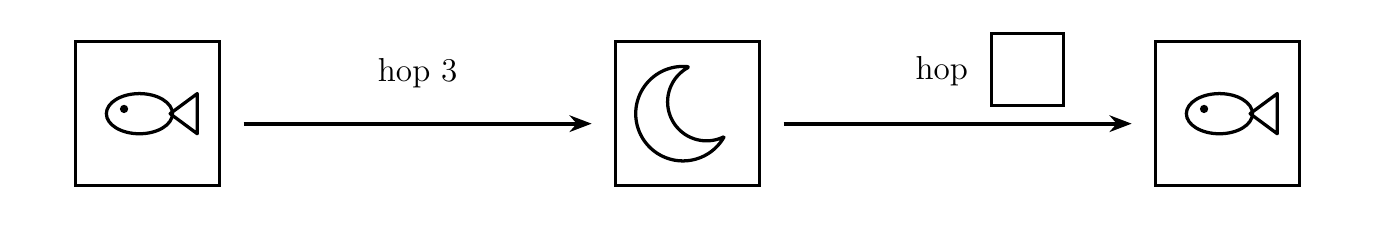
\begin{tikzpicture}[x=1in,y=1in]
\useasboundingbox (0,-0.42) rectangle (6.6,0.43);
\draw[line width=1.2pt] (0.24,-0.36) rectangle (0.96,0.36);
\draw[line width=1.18pt] (0.5587,0) ellipse (0.1653 and 0.1004);
\draw[line width=1.18pt, line join=round] (0.7122,0) -- (0.848,0.1004) -- (0.848,-0.1004) -- cycle;
\fill (0.4819,0.0236) circle (0.0207);
\draw[line width=1.2pt] (2.94,-0.36) rectangle (3.66,0.36);
\draw[line width=1.18pt, line join=round] (3.3011,0.2349) -- (3.2929,0.2356) -- (3.2846,0.236) -- (3.2764,0.2362) -- (3.2681,0.236) -- (3.2599,0.2356) -- (3.2517,0.2349) -- (3.2435,0.2339) -- (3.2354,0.2326) -- (3.2273,0.231) -- (3.2193,0.2291) -- (3.2113,0.227) -- (3.2034,0.2246) -- (3.1956,0.2219) -- (3.1879,0.219) -- (3.1803,0.2157) -- (3.1729,0.2123) -- (3.1655,0.2085) -- (3.1583,0.2045) -- (3.1512,0.2003) -- (3.1443,0.1958) -- (3.1376,0.1911) -- (3.131,0.1861) -- (3.1246,0.1809) -- (3.1184,0.1755) -- (3.1123,0.1699) -- (3.1065,0.1641) -- (3.1009,0.158) -- (3.0955,0.1518) -- (3.0903,0.1454) -- (3.0853,0.1388) -- (3.0806,0.1321) -- (3.0761,0.1251) -- (3.0719,0.1181) -- (3.0679,0.1109) -- (3.0641,0.1035) -- (3.0606,0.0961) -- (3.0574,0.0885) -- (3.0545,0.0808) -- (3.0518,0.073) -- (3.0494,0.0651) -- (3.0472,0.0571) -- (3.0454,0.0491) -- (3.0438,0.041) -- (3.0425,0.0329) -- (3.0415,0.0247) -- (3.0408,0.0165) -- (3.0404,0.0082) -- (3.0402,0) -- (3.0404,-0.0082) -- (3.0408,-0.0165) -- (3.0415,-0.0247) -- (3.0425,-0.0329) -- (3.0438,-0.041) -- (3.0454,-0.0491) -- (3.0472,-0.0571) -- (3.0494,-0.0651) -- (3.0518,-0.073) -- (3.0545,-0.0808) -- (3.0574,-0.0885) -- (3.0606,-0.0961) -- (3.0641,-0.1035) -- (3.0679,-0.1109) -- (3.0719,-0.1181) -- (3.0761,-0.1251) -- (3.0806,-0.1321) -- (3.0853,-0.1388) -- (3.0903,-0.1454) -- (3.0955,-0.1518) -- (3.1009,-0.158) -- (3.1065,-0.1641) -- (3.1123,-0.1699) -- (3.1184,-0.1755) -- (3.1246,-0.1809) -- (3.131,-0.1861) -- (3.1376,-0.1911) -- (3.1443,-0.1958) -- (3.1512,-0.2003) -- (3.1583,-0.2045) -- (3.1655,-0.2085) -- (3.1729,-0.2123) -- (3.1803,-0.2157) -- (3.1879,-0.219) -- (3.1956,-0.2219) -- (3.2034,-0.2246) -- (3.2113,-0.227) -- (3.2193,-0.2291) -- (3.2273,-0.231) -- (3.2354,-0.2326) -- (3.2435,-0.2339) -- (3.2517,-0.2349) -- (3.2599,-0.2356) -- (3.2681,-0.236) -- (3.2764,-0.2362) -- (3.2846,-0.236) -- (3.2929,-0.2356) -- (3.3011,-0.2349) -- (3.3093,-0.2339) -- (3.3174,-0.2326) -- (3.3255,-0.231) -- (3.3335,-0.2291) -- (3.3415,-0.227) -- (3.3494,-0.2246) -- (3.3572,-0.2219) -- (3.3649,-0.219) -- (3.3724,-0.2157) -- (3.3799,-0.2123) -- (3.3873,-0.2085) -- (3.3945,-0.2045) -- (3.4015,-0.2003) -- (3.4084,-0.1958) -- (3.4152,-0.1911) -- (3.4218,-0.1861) -- (3.4282,-0.1809) -- (3.4344,-0.1755) -- (3.4404,-0.1699) -- (3.4463,-0.1641) -- (3.4519,-0.158) -- (3.4573,-0.1518) -- (3.4625,-0.1454) -- (3.4674,-0.1388) -- (3.4722,-0.1321) -- (3.4767,-0.1251) -- (3.4809,-0.1181) -- (3.4799,-0.1161) -- (3.4737,-0.1189) -- (3.4674,-0.1216) -- (3.4611,-0.124) -- (3.4547,-0.1263) -- (3.4482,-0.1282) -- (3.4416,-0.13) -- (3.435,-0.1315) -- (3.4283,-0.1328) -- (3.4216,-0.1339) -- (3.4148,-0.1347) -- (3.4081,-0.1353) -- (3.4013,-0.1357) -- (3.3945,-0.1358) -- (3.3877,-0.1357) -- (3.3809,-0.1353) -- (3.3741,-0.1347) -- (3.3673,-0.1339) -- (3.3606,-0.1328) -- (3.354,-0.1315) -- (3.3473,-0.13) -- (3.3408,-0.1282) -- (3.3343,-0.1263) -- (3.3278,-0.124) -- (3.3215,-0.1216) -- (3.3152,-0.1189) -- (3.3091,-0.1161) -- (3.303,-0.113) -- (3.297,-0.1097) -- (3.2912,-0.1062) -- (3.2855,-0.1025) -- (3.2799,-0.0986) -- (3.2745,-0.0945) -- (3.2692,-0.0902) -- (3.2641,-0.0857) -- (3.2591,-0.0811) -- (3.2543,-0.0763) -- (3.2497,-0.0713) -- (3.2452,-0.0662) -- (3.2409,-0.0609) -- (3.2368,-0.0555) -- (3.2329,-0.0499) -- (3.2292,-0.0442) -- (3.2257,-0.0384) -- (3.2224,-0.0324) -- (3.2194,-0.0264) -- (3.2165,-0.0202) -- (3.2138,-0.0139) -- (3.2114,-0.0076) -- (3.2092,-0.0012) -- (3.2072,0.0053) -- (3.2054,0.0119) -- (3.2039,0.0185) -- (3.2026,0.0252) -- (3.2015,0.0319) -- (3.2007,0.0387) -- (3.2001,0.0454) -- (3.1998,0.0522) -- (3.1996,0.059) -- (3.1998,0.0658) -- (3.2001,0.0726) -- (3.2007,0.0794) -- (3.2015,0.0862) -- (3.2026,0.0929) -- (3.2039,0.0995) -- (3.2054,0.1062) -- (3.2072,0.1127) -- (3.2092,0.1192) -- (3.2114,0.1257) -- (3.2138,0.132) -- (3.2165,0.1383) -- (3.2194,0.1444) -- (3.2224,0.1505) -- (3.2257,0.1565) -- (3.2292,0.1623) -- (3.2329,0.168) -- (3.2368,0.1736) -- (3.2409,0.179) -- (3.2452,0.1843) -- (3.2497,0.1894) -- (3.2543,0.1944) -- (3.2591,0.1992) -- (3.2641,0.2038) -- (3.2692,0.2083) -- (3.2745,0.2126) -- (3.2799,0.2167) -- (3.2855,0.2206) -- (3.2912,0.2243) -- (3.297,0.2278) -- (3.303,0.2311) -- cycle;
\draw[line width=1.2pt] (5.64,-0.36) rectangle (6.36,0.36);
\draw[line width=1.18pt] (5.9587,0) ellipse (0.1653 and 0.1004);
\draw[line width=1.18pt, line join=round] (6.1122,0) -- (6.248,0.1004) -- (6.248,-0.1004) -- cycle;
\fill (5.8819,0.0236) circle (0.0207);
\draw[line width=1.4pt, -{Stealth[length=8pt]}] (1.08,-0.05) -- (2.82,-0.05);
\node[font=\large] at (1.95,0.2) {hop 3};
\draw[line width=1.4pt, -{Stealth[length=8pt]}] (3.78,-0.05) -- (5.52,-0.05);
\node[font=\large, anchor=east] at (4.75,0.21) {hop};
\draw[line width=1pt] (4.82,0.04) rectangle (5.18,0.4);
\end{tikzpicture}}\par
\par\vspace{0.18in}\noindent\makebox[\textwidth][c]{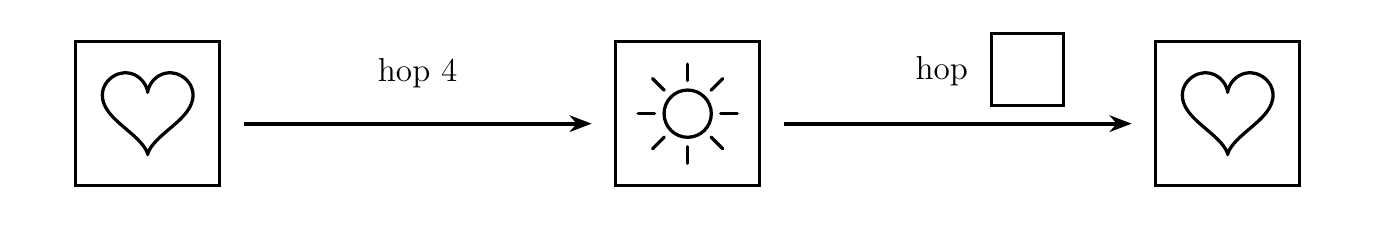
\begin{tikzpicture}[x=1in,y=1in]
\useasboundingbox (0,-0.42) rectangle (6.6,0.43);
\draw[line width=1.2pt] (0.24,-0.36) rectangle (0.96,0.36);
\draw[line width=1.18pt, line join=round] (0.6,0.1063) -- (0.6,0.1071) -- (0.6003,0.1094) -- (0.6009,0.1133) -- (0.602,0.1185) -- (0.6039,0.1249) -- (0.6067,0.1323) -- (0.6104,0.1404) -- (0.6153,0.149) -- (0.6212,0.1579) -- (0.6283,0.1666) -- (0.6366,0.175) -- (0.646,0.1828) -- (0.6565,0.1897) -- (0.6679,0.1954) -- (0.6802,0.1999) -- (0.693,0.2029) -- (0.7064,0.2043) -- (0.72,0.204) -- (0.7337,0.202) -- (0.7473,0.1984) -- (0.7604,0.1931) -- (0.7728,0.1862) -- (0.7845,0.1779) -- (0.795,0.1682) -- (0.8043,0.1574) -- (0.8122,0.1456) -- (0.8184,0.133) -- (0.823,0.1198) -- (0.8258,0.1061) -- (0.8267,0.0921) -- (0.8258,0.078) -- (0.823,0.0638) -- (0.8184,0.0497) -- (0.8122,0.0357) -- (0.8043,0.022) -- (0.795,0.0085) -- (0.7845,-0.0047) -- (0.7728,-0.0176) -- (0.7604,-0.0302) -- (0.7473,-0.0425) -- (0.7337,-0.0546) -- (0.72,-0.0664) -- (0.7064,-0.0781) -- (0.693,-0.0895) -- (0.6802,-0.1007) -- (0.6679,-0.1117) -- (0.6565,-0.1224) -- (0.646,-0.1328) -- (0.6366,-0.1428) -- (0.6283,-0.1524) -- (0.6212,-0.1615) -- (0.6153,-0.17) -- (0.6104,-0.1778) -- (0.6067,-0.1848) -- (0.6039,-0.1909) -- (0.602,-0.196) -- (0.6009,-0.2001) -- (0.6003,-0.2031) -- (0.6,-0.2049) -- (0.6,-0.2055) -- (0.6,-0.2049) -- (0.5997,-0.2031) -- (0.5991,-0.2001) -- (0.598,-0.196) -- (0.5961,-0.1909) -- (0.5933,-0.1848) -- (0.5896,-0.1778) -- (0.5847,-0.17) -- (0.5788,-0.1615) -- (0.5717,-0.1524) -- (0.5634,-0.1428) -- (0.554,-0.1328) -- (0.5435,-0.1224) -- (0.5321,-0.1117) -- (0.5198,-0.1007) -- (0.507,-0.0895) -- (0.4936,-0.0781) -- (0.48,-0.0664) -- (0.4663,-0.0546) -- (0.4527,-0.0425) -- (0.4396,-0.0302) -- (0.4272,-0.0176) -- (0.4155,-0.0047) -- (0.405,0.0085) -- (0.3957,0.022) -- (0.3878,0.0357) -- (0.3816,0.0497) -- (0.377,0.0638) -- (0.3742,0.078) -- (0.3733,0.0921) -- (0.3742,0.1061) -- (0.377,0.1198) -- (0.3816,0.133) -- (0.3878,0.1456) -- (0.3957,0.1574) -- (0.405,0.1682) -- (0.4155,0.1779) -- (0.4272,0.1862) -- (0.4396,0.1931) -- (0.4527,0.1984) -- (0.4663,0.202) -- (0.48,0.204) -- (0.4936,0.2043) -- (0.507,0.2029) -- (0.5198,0.1999) -- (0.5321,0.1954) -- (0.5435,0.1897) -- (0.554,0.1828) -- (0.5634,0.175) -- (0.5717,0.1666) -- (0.5788,0.1579) -- (0.5847,0.149) -- (0.5896,0.1404) -- (0.5933,0.1323) -- (0.5961,0.1249) -- (0.598,0.1185) -- (0.5991,0.1133) -- (0.5997,0.1094) -- (0.6,0.1071) -- cycle;
\draw[line width=1.2pt] (2.94,-0.36) rectangle (3.66,0.36);
\draw[line width=1.18pt] (3.3,0) circle (0.1181);
\draw[line width=1.18pt, line cap=round] (3.4653,0) -- (3.548,0);
\draw[line width=1.18pt, line cap=round] (3.4169,0.1169) -- (3.4753,0.1753);
\draw[line width=1.18pt, line cap=round] (3.3,0.1653) -- (3.3,0.248);
\draw[line width=1.18pt, line cap=round] (3.1831,0.1169) -- (3.1247,0.1753);
\draw[line width=1.18pt, line cap=round] (3.1347,0) -- (3.052,0);
\draw[line width=1.18pt, line cap=round] (3.1831,-0.1169) -- (3.1247,-0.1753);
\draw[line width=1.18pt, line cap=round] (3.3,-0.1653) -- (3.3,-0.248);
\draw[line width=1.18pt, line cap=round] (3.4169,-0.1169) -- (3.4753,-0.1753);
\draw[line width=1.2pt] (5.64,-0.36) rectangle (6.36,0.36);
\draw[line width=1.18pt, line join=round] (6,0.1063) -- (6,0.1071) -- (6.0003,0.1094) -- (6.0009,0.1133) -- (6.002,0.1185) -- (6.0039,0.1249) -- (6.0067,0.1323) -- (6.0104,0.1404) -- (6.0153,0.149) -- (6.0212,0.1579) -- (6.0283,0.1666) -- (6.0366,0.175) -- (6.046,0.1828) -- (6.0565,0.1897) -- (6.0679,0.1954) -- (6.0802,0.1999) -- (6.093,0.2029) -- (6.1064,0.2043) -- (6.12,0.204) -- (6.1337,0.202) -- (6.1473,0.1984) -- (6.1604,0.1931) -- (6.1728,0.1862) -- (6.1845,0.1779) -- (6.195,0.1682) -- (6.2043,0.1574) -- (6.2122,0.1456) -- (6.2184,0.133) -- (6.223,0.1198) -- (6.2258,0.1061) -- (6.2267,0.0921) -- (6.2258,0.078) -- (6.223,0.0638) -- (6.2184,0.0497) -- (6.2122,0.0357) -- (6.2043,0.022) -- (6.195,0.0085) -- (6.1845,-0.0047) -- (6.1728,-0.0176) -- (6.1604,-0.0302) -- (6.1473,-0.0425) -- (6.1337,-0.0546) -- (6.12,-0.0664) -- (6.1064,-0.0781) -- (6.093,-0.0895) -- (6.0802,-0.1007) -- (6.0679,-0.1117) -- (6.0565,-0.1224) -- (6.046,-0.1328) -- (6.0366,-0.1428) -- (6.0283,-0.1524) -- (6.0212,-0.1615) -- (6.0153,-0.17) -- (6.0104,-0.1778) -- (6.0067,-0.1848) -- (6.0039,-0.1909) -- (6.002,-0.196) -- (6.0009,-0.2001) -- (6.0003,-0.2031) -- (6,-0.2049) -- (6,-0.2055) -- (6,-0.2049) -- (5.9997,-0.2031) -- (5.9991,-0.2001) -- (5.998,-0.196) -- (5.9961,-0.1909) -- (5.9933,-0.1848) -- (5.9896,-0.1778) -- (5.9847,-0.17) -- (5.9788,-0.1615) -- (5.9717,-0.1524) -- (5.9634,-0.1428) -- (5.954,-0.1328) -- (5.9435,-0.1224) -- (5.9321,-0.1117) -- (5.9198,-0.1007) -- (5.907,-0.0895) -- (5.8936,-0.0781) -- (5.88,-0.0664) -- (5.8663,-0.0546) -- (5.8527,-0.0425) -- (5.8396,-0.0302) -- (5.8272,-0.0176) -- (5.8155,-0.0047) -- (5.805,0.0085) -- (5.7957,0.022) -- (5.7878,0.0357) -- (5.7816,0.0497) -- (5.777,0.0638) -- (5.7742,0.078) -- (5.7733,0.0921) -- (5.7742,0.1061) -- (5.777,0.1198) -- (5.7816,0.133) -- (5.7878,0.1456) -- (5.7957,0.1574) -- (5.805,0.1682) -- (5.8155,0.1779) -- (5.8272,0.1862) -- (5.8396,0.1931) -- (5.8527,0.1984) -- (5.8663,0.202) -- (5.88,0.204) -- (5.8936,0.2043) -- (5.907,0.2029) -- (5.9198,0.1999) -- (5.9321,0.1954) -- (5.9435,0.1897) -- (5.954,0.1828) -- (5.9634,0.175) -- (5.9717,0.1666) -- (5.9788,0.1579) -- (5.9847,0.149) -- (5.9896,0.1404) -- (5.9933,0.1323) -- (5.9961,0.1249) -- (5.998,0.1185) -- (5.9991,0.1133) -- (5.9997,0.1094) -- (6,0.1071) -- cycle;
\draw[line width=1.4pt, -{Stealth[length=8pt]}] (1.08,-0.05) -- (2.82,-0.05);
\node[font=\large] at (1.95,0.2) {hop 4};
\draw[line width=1.4pt, -{Stealth[length=8pt]}] (3.78,-0.05) -- (5.52,-0.05);
\node[font=\large, anchor=east] at (4.75,0.21) {hop};
\draw[line width=1pt] (4.82,0.04) rectangle (5.18,0.4);
\end{tikzpicture}}\par
\vfill

\newpage
\par\vspace{0in}\noindent \prob{10} A secret hop changed the sun into the tree. Draw what the same hop changes each of these pictures into.\par
\par\vspace{0.25in}\noindent\makebox[\textwidth][c]{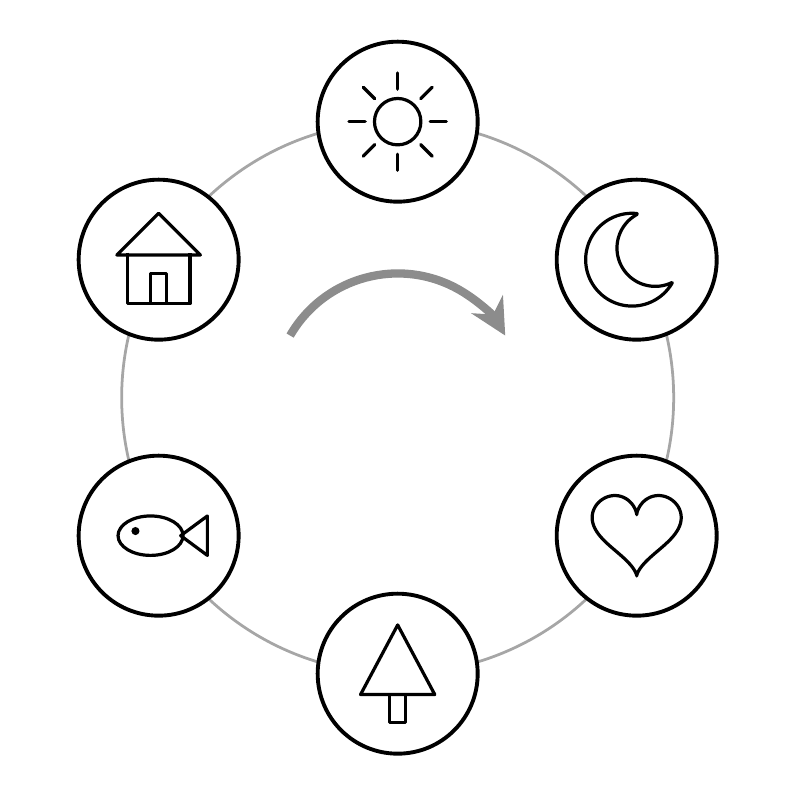
\begin{tikzpicture}[x=1in,y=1in]
\useasboundingbox (-1.85,-1.85) rectangle (1.85,1.85);
\draw[black!35, line width=1pt] (0,0) circle (1.38);
\filldraw[fill=white, draw=black, line width=1.4pt] (0,1.38) circle (0.4);
\draw[line width=1.16pt] (0,1.38) circle (0.116);
\draw[line width=1.16pt, line cap=round] (0.1624,1.38) -- (0.2436,1.38);
\draw[line width=1.16pt, line cap=round] (0.1148,1.4948) -- (0.1723,1.5523);
\draw[line width=1.16pt, line cap=round] (0,1.5424) -- (0,1.6236);
\draw[line width=1.16pt, line cap=round] (-0.1148,1.4948) -- (-0.1723,1.5523);
\draw[line width=1.16pt, line cap=round] (-0.1624,1.38) -- (-0.2436,1.38);
\draw[line width=1.16pt, line cap=round] (-0.1148,1.2652) -- (-0.1723,1.2077);
\draw[line width=1.16pt, line cap=round] (0,1.2176) -- (0,1.1364);
\draw[line width=1.16pt, line cap=round] (0.1148,1.2652) -- (0.1723,1.2077);
\filldraw[fill=white, draw=black, line width=1.4pt] (1.1951,0.69) circle (0.4);
\draw[line width=1.16pt, line join=round] (1.1962,0.9207) -- (1.1881,0.9214) -- (1.18,0.9219) -- (1.1719,0.922) -- (1.1638,0.9219) -- (1.1557,0.9214) -- (1.1477,0.9207) -- (1.1396,0.9197) -- (1.1316,0.9185) -- (1.1237,0.9169) -- (1.1158,0.9151) -- (1.108,0.913) -- (1.1002,0.9106) -- (1.0926,0.908) -- (1.085,0.9051) -- (1.0776,0.9019) -- (1.0702,0.8985) -- (1.063,0.8948) -- (1.0559,0.8909) -- (1.049,0.8867) -- (1.0422,0.8823) -- (1.0355,0.8777) -- (1.0291,0.8728) -- (1.0228,0.8677) -- (1.0167,0.8624) -- (1.0108,0.8569) -- (1.005,0.8512) -- (0.9995,0.8452) -- (0.9942,0.8391) -- (0.9891,0.8328) -- (0.9842,0.8264) -- (0.9796,0.8197) -- (0.9752,0.8129) -- (0.971,0.806) -- (0.9671,0.7989) -- (0.9634,0.7917) -- (0.96,0.7844) -- (0.9568,0.7769) -- (0.9539,0.7693) -- (0.9513,0.7617) -- (0.9489,0.7539) -- (0.9468,0.7461) -- (0.945,0.7382) -- (0.9434,0.7303) -- (0.9422,0.7223) -- (0.9412,0.7143) -- (0.9405,0.7062) -- (0.9401,0.6981) -- (0.9399,0.69) -- (0.9401,0.6819) -- (0.9405,0.6738) -- (0.9412,0.6657) -- (0.9422,0.6577) -- (0.9434,0.6497) -- (0.945,0.6418) -- (0.9468,0.6339) -- (0.9489,0.6261) -- (0.9513,0.6183) -- (0.9539,0.6107) -- (0.9568,0.6031) -- (0.96,0.5956) -- (0.9634,0.5883) -- (0.9671,0.5811) -- (0.971,0.574) -- (0.9752,0.5671) -- (0.9796,0.5603) -- (0.9842,0.5536) -- (0.9891,0.5472) -- (0.9942,0.5409) -- (0.9995,0.5348) -- (1.005,0.5288) -- (1.0108,0.5231) -- (1.0167,0.5176) -- (1.0228,0.5123) -- (1.0291,0.5072) -- (1.0355,0.5023) -- (1.0422,0.4977) -- (1.049,0.4933) -- (1.0559,0.4891) -- (1.063,0.4852) -- (1.0702,0.4815) -- (1.0776,0.4781) -- (1.085,0.4749) -- (1.0926,0.472) -- (1.1002,0.4694) -- (1.108,0.467) -- (1.1158,0.4649) -- (1.1237,0.4631) -- (1.1316,0.4615) -- (1.1396,0.4603) -- (1.1477,0.4593) -- (1.1557,0.4586) -- (1.1638,0.4581) -- (1.1719,0.458) -- (1.18,0.4581) -- (1.1881,0.4586) -- (1.1962,0.4593) -- (1.2042,0.4603) -- (1.2122,0.4615) -- (1.2202,0.4631) -- (1.228,0.4649) -- (1.2359,0.467) -- (1.2436,0.4694) -- (1.2513,0.472) -- (1.2588,0.4749) -- (1.2663,0.4781) -- (1.2736,0.4815) -- (1.2808,0.4852) -- (1.2879,0.4891) -- (1.2949,0.4933) -- (1.3016,0.4977) -- (1.3083,0.5023) -- (1.3147,0.5072) -- (1.321,0.5123) -- (1.3272,0.5176) -- (1.3331,0.5231) -- (1.3388,0.5288) -- (1.3443,0.5348) -- (1.3496,0.5409) -- (1.3547,0.5472) -- (1.3596,0.5536) -- (1.3643,0.5603) -- (1.3687,0.5671) -- (1.3728,0.574) -- (1.3718,0.576) -- (1.3658,0.5731) -- (1.3596,0.5705) -- (1.3534,0.5681) -- (1.3471,0.566) -- (1.3407,0.564) -- (1.3342,0.5623) -- (1.3277,0.5608) -- (1.3212,0.5595) -- (1.3146,0.5585) -- (1.3079,0.5576) -- (1.3013,0.5571) -- (1.2946,0.5567) -- (1.2879,0.5566) -- (1.2812,0.5567) -- (1.2746,0.5571) -- (1.2679,0.5576) -- (1.2613,0.5585) -- (1.2547,0.5595) -- (1.2481,0.5608) -- (1.2416,0.5623) -- (1.2352,0.564) -- (1.2288,0.566) -- (1.2225,0.5681) -- (1.2162,0.5705) -- (1.2101,0.5731) -- (1.204,0.576) -- (1.1981,0.579) -- (1.1922,0.5822) -- (1.1865,0.5857) -- (1.1809,0.5893) -- (1.1754,0.5932) -- (1.1701,0.5972) -- (1.1649,0.6014) -- (1.1598,0.6058) -- (1.155,0.6103) -- (1.1502,0.615) -- (1.1457,0.6199) -- (1.1413,0.625) -- (1.1371,0.6302) -- (1.1331,0.6355) -- (1.1292,0.641) -- (1.1256,0.6466) -- (1.1222,0.6523) -- (1.1189,0.6581) -- (1.1159,0.6641) -- (1.1131,0.6702) -- (1.1105,0.6763) -- (1.1081,0.6825) -- (1.1059,0.6889) -- (1.1039,0.6952) -- (1.1022,0.7017) -- (1.1007,0.7082) -- (1.0994,0.7148) -- (1.0984,0.7214) -- (1.0976,0.728) -- (1.097,0.7346) -- (1.0966,0.7413) -- (1.0965,0.748) -- (1.0966,0.7547) -- (1.097,0.7614) -- (1.0976,0.768) -- (1.0984,0.7746) -- (1.0994,0.7812) -- (1.1007,0.7878) -- (1.1022,0.7943) -- (1.1039,0.8008) -- (1.1059,0.8071) -- (1.1081,0.8135) -- (1.1105,0.8197) -- (1.1131,0.8258) -- (1.1159,0.8319) -- (1.1189,0.8379) -- (1.1222,0.8437) -- (1.1256,0.8494) -- (1.1292,0.855) -- (1.1331,0.8605) -- (1.1371,0.8658) -- (1.1413,0.871) -- (1.1457,0.8761) -- (1.1502,0.881) -- (1.155,0.8857) -- (1.1598,0.8902) -- (1.1649,0.8946) -- (1.1701,0.8988) -- (1.1754,0.9028) -- (1.1809,0.9067) -- (1.1865,0.9103) -- (1.1922,0.9138) -- (1.1981,0.917) -- cycle;
\filldraw[fill=white, draw=black, line width=1.4pt] (1.1951,-0.69) circle (0.4);
\draw[line width=1.16pt, line join=round] (1.1951,-0.5856) -- (1.1951,-0.5848) -- (1.1954,-0.5825) -- (1.196,-0.5787) -- (1.1971,-0.5736) -- (1.199,-0.5673) -- (1.2017,-0.5601) -- (1.2054,-0.5521) -- (1.2101,-0.5436) -- (1.216,-0.5349) -- (1.223,-0.5263) -- (1.2311,-0.5181) -- (1.2403,-0.5104) -- (1.2506,-0.5037) -- (1.2618,-0.498) -- (1.2739,-0.4936) -- (1.2865,-0.4907) -- (1.2997,-0.4893) -- (1.313,-0.4896) -- (1.3265,-0.4915) -- (1.3398,-0.4951) -- (1.3527,-0.5003) -- (1.3649,-0.5071) -- (1.3763,-0.5153) -- (1.3867,-0.5248) -- (1.3958,-0.5354) -- (1.4036,-0.5469) -- (1.4097,-0.5593) -- (1.4142,-0.5723) -- (1.4169,-0.5858) -- (1.4178,-0.5995) -- (1.4169,-0.6134) -- (1.4142,-0.6274) -- (1.4097,-0.6412) -- (1.4036,-0.6549) -- (1.3958,-0.6684) -- (1.3867,-0.6816) -- (1.3763,-0.6946) -- (1.3649,-0.7073) -- (1.3527,-0.7196) -- (1.3398,-0.7318) -- (1.3265,-0.7436) -- (1.313,-0.7553) -- (1.2997,-0.7667) -- (1.2865,-0.7779) -- (1.2739,-0.7889) -- (1.2618,-0.7997) -- (1.2506,-0.8102) -- (1.2403,-0.8204) -- (1.2311,-0.8303) -- (1.223,-0.8398) -- (1.216,-0.8487) -- (1.2101,-0.857) -- (1.2054,-0.8647) -- (1.2017,-0.8715) -- (1.199,-0.8775) -- (1.1971,-0.8826) -- (1.196,-0.8866) -- (1.1954,-0.8895) -- (1.1951,-0.8912) -- (1.1951,-0.8918) -- (1.1951,-0.8912) -- (1.1949,-0.8895) -- (1.1943,-0.8866) -- (1.1931,-0.8826) -- (1.1913,-0.8775) -- (1.1885,-0.8715) -- (1.1849,-0.8647) -- (1.1801,-0.857) -- (1.1743,-0.8487) -- (1.1673,-0.8398) -- (1.1591,-0.8303) -- (1.1499,-0.8204) -- (1.1396,-0.8102) -- (1.1284,-0.7997) -- (1.1164,-0.7889) -- (1.1037,-0.7779) -- (1.0906,-0.7667) -- (1.0772,-0.7553) -- (1.0637,-0.7436) -- (1.0505,-0.7318) -- (1.0376,-0.7196) -- (1.0253,-0.7073) -- (1.0139,-0.6946) -- (1.0035,-0.6816) -- (0.9944,-0.6684) -- (0.9867,-0.6549) -- (0.9805,-0.6412) -- (0.976,-0.6274) -- (0.9733,-0.6134) -- (0.9724,-0.5995) -- (0.9733,-0.5858) -- (0.976,-0.5723) -- (0.9805,-0.5593) -- (0.9867,-0.5469) -- (0.9944,-0.5354) -- (1.0035,-0.5248) -- (1.0139,-0.5153) -- (1.0253,-0.5071) -- (1.0376,-0.5003) -- (1.0505,-0.4951) -- (1.0637,-0.4915) -- (1.0772,-0.4896) -- (1.0906,-0.4893) -- (1.1037,-0.4907) -- (1.1164,-0.4936) -- (1.1284,-0.498) -- (1.1396,-0.5037) -- (1.1499,-0.5104) -- (1.1591,-0.5181) -- (1.1673,-0.5263) -- (1.1743,-0.5349) -- (1.1801,-0.5436) -- (1.1849,-0.5521) -- (1.1885,-0.5601) -- (1.1913,-0.5673) -- (1.1931,-0.5736) -- (1.1943,-0.5787) -- (1.1949,-0.5825) -- (1.1951,-0.5848) -- cycle;
\filldraw[fill=white, draw=black, line width=1.4pt] (0,-1.38) circle (0.4);
\draw[line width=1.16pt, line join=round] (-0.1856,-1.4844) -- (0,-1.1364) -- (0.1856,-1.4844) -- cycle;
\draw[line width=1.16pt, line join=round] (-0.0406,-1.4844) -- (-0.0406,-1.6236) -- (0.0406,-1.6236) -- (0.0406,-1.4844);
\filldraw[fill=white, draw=black, line width=1.4pt] (-1.1951,-0.69) circle (0.4);
\draw[line width=1.16pt] (-1.2357,-0.69) ellipse (0.1624 and 0.0986);
\draw[line width=1.16pt, line join=round] (-1.0849,-0.69) -- (-0.9515,-0.5914) -- (-0.9515,-0.7886) -- cycle;
\fill (-1.3111,-0.6668) circle (0.0203);
\filldraw[fill=white, draw=black, line width=1.4pt] (-1.1951,0.69) circle (0.4);
\draw[line width=1.16pt, line join=round] (-1.3517,0.7248) -- (-1.3517,0.4696) -- (-1.0385,0.4696) -- (-1.0385,0.7248);
\draw[line width=1.16pt, line join=round] (-1.4039,0.7132) -- (-1.1951,0.922) -- (-0.9863,0.7132) -- cycle;
\draw[line width=1.16pt, line join=round] (-1.2357,0.4696) -- (-1.2357,0.6204) -- (-1.1545,0.6204) -- (-1.1545,0.4696);
\draw[black!45, line width=3pt, -{Stealth[length=13pt, width=13pt]}] (-0.5378,0.3105) arc[start angle=150, end angle=30, radius=0.621];
\end{tikzpicture}}\par
\par\vspace{0.35in}\noindent\makebox[\textwidth][c]{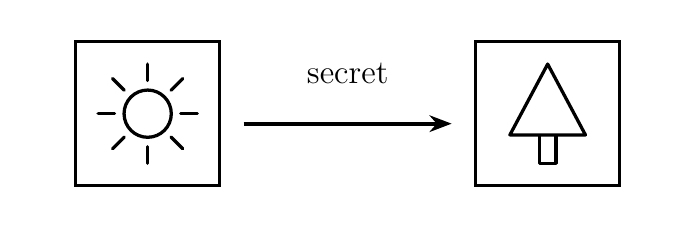
\begin{tikzpicture}[x=1in,y=1in]
\useasboundingbox (0,-0.42) rectangle (3.2,0.43);
\draw[line width=1.2pt] (0.24,-0.36) rectangle (0.96,0.36);
\draw[line width=1.18pt] (0.6,0) circle (0.1181);
\draw[line width=1.18pt, line cap=round] (0.7653,0) -- (0.848,0);
\draw[line width=1.18pt, line cap=round] (0.7169,0.1169) -- (0.7753,0.1753);
\draw[line width=1.18pt, line cap=round] (0.6,0.1653) -- (0.6,0.248);
\draw[line width=1.18pt, line cap=round] (0.4831,0.1169) -- (0.4247,0.1753);
\draw[line width=1.18pt, line cap=round] (0.4347,0) -- (0.352,0);
\draw[line width=1.18pt, line cap=round] (0.4831,-0.1169) -- (0.4247,-0.1753);
\draw[line width=1.18pt, line cap=round] (0.6,-0.1653) -- (0.6,-0.248);
\draw[line width=1.18pt, line cap=round] (0.7169,-0.1169) -- (0.7753,-0.1753);
\draw[line width=1.2pt] (2.24,-0.36) rectangle (2.96,0.36);
\draw[line width=1.18pt, line join=round] (2.4111,-0.1063) -- (2.6,0.248) -- (2.7889,-0.1063) -- cycle;
\draw[line width=1.18pt, line join=round] (2.5587,-0.1063) -- (2.5587,-0.248) -- (2.6413,-0.248) -- (2.6413,-0.1063);
\draw[line width=1.4pt, -{Stealth[length=8pt]}] (1.08,-0.05) -- (2.12,-0.05);
\node[font=\large] at (1.6,0.2) {secret};
\end{tikzpicture}}\par
\par\vspace{0.3in}\noindent\makebox[\textwidth][c]{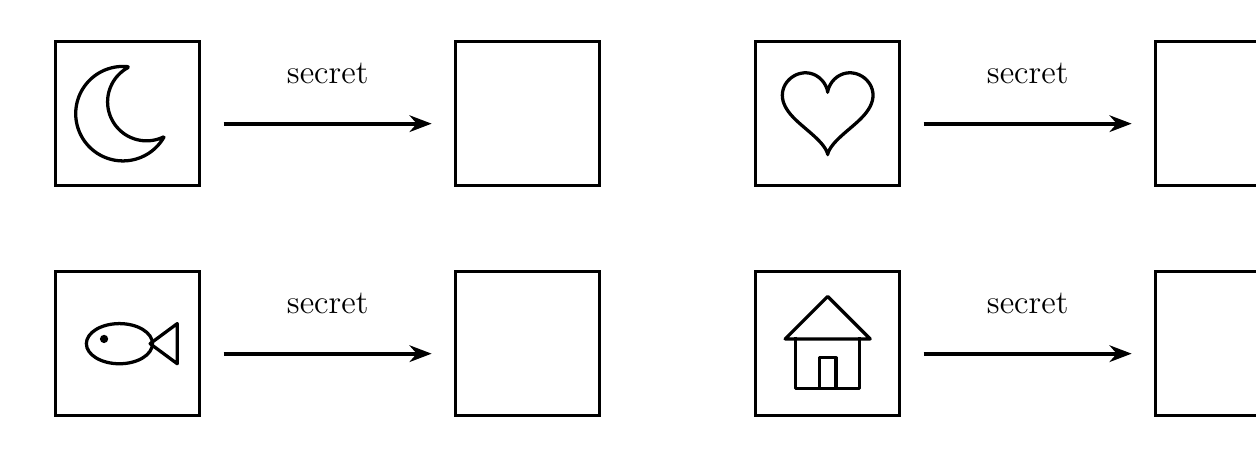
\begin{tikzpicture}[x=1in,y=1in]
\useasboundingbox (0,-1.57) rectangle (6,0.43);
\draw[line width=1.2pt] (0.14,-0.36) rectangle (0.86,0.36);
\draw[line width=1.18pt, line join=round] (0.5011,0.2349) -- (0.4929,0.2356) -- (0.4846,0.236) -- (0.4764,0.2362) -- (0.4681,0.236) -- (0.4599,0.2356) -- (0.4517,0.2349) -- (0.4435,0.2339) -- (0.4354,0.2326) -- (0.4273,0.231) -- (0.4193,0.2291) -- (0.4113,0.227) -- (0.4034,0.2246) -- (0.3956,0.2219) -- (0.3879,0.219) -- (0.3803,0.2157) -- (0.3729,0.2123) -- (0.3655,0.2085) -- (0.3583,0.2045) -- (0.3512,0.2003) -- (0.3443,0.1958) -- (0.3376,0.1911) -- (0.331,0.1861) -- (0.3246,0.1809) -- (0.3184,0.1755) -- (0.3123,0.1699) -- (0.3065,0.1641) -- (0.3009,0.158) -- (0.2955,0.1518) -- (0.2903,0.1454) -- (0.2853,0.1388) -- (0.2806,0.1321) -- (0.2761,0.1251) -- (0.2719,0.1181) -- (0.2679,0.1109) -- (0.2641,0.1035) -- (0.2606,0.0961) -- (0.2574,0.0885) -- (0.2545,0.0808) -- (0.2518,0.073) -- (0.2494,0.0651) -- (0.2472,0.0571) -- (0.2454,0.0491) -- (0.2438,0.041) -- (0.2425,0.0329) -- (0.2415,0.0247) -- (0.2408,0.0165) -- (0.2404,0.0082) -- (0.2402,0) -- (0.2404,-0.0082) -- (0.2408,-0.0165) -- (0.2415,-0.0247) -- (0.2425,-0.0329) -- (0.2438,-0.041) -- (0.2454,-0.0491) -- (0.2472,-0.0571) -- (0.2494,-0.0651) -- (0.2518,-0.073) -- (0.2545,-0.0808) -- (0.2574,-0.0885) -- (0.2606,-0.0961) -- (0.2641,-0.1035) -- (0.2679,-0.1109) -- (0.2719,-0.1181) -- (0.2761,-0.1251) -- (0.2806,-0.1321) -- (0.2853,-0.1388) -- (0.2903,-0.1454) -- (0.2955,-0.1518) -- (0.3009,-0.158) -- (0.3065,-0.1641) -- (0.3123,-0.1699) -- (0.3184,-0.1755) -- (0.3246,-0.1809) -- (0.331,-0.1861) -- (0.3376,-0.1911) -- (0.3443,-0.1958) -- (0.3512,-0.2003) -- (0.3583,-0.2045) -- (0.3655,-0.2085) -- (0.3729,-0.2123) -- (0.3803,-0.2157) -- (0.3879,-0.219) -- (0.3956,-0.2219) -- (0.4034,-0.2246) -- (0.4113,-0.227) -- (0.4193,-0.2291) -- (0.4273,-0.231) -- (0.4354,-0.2326) -- (0.4435,-0.2339) -- (0.4517,-0.2349) -- (0.4599,-0.2356) -- (0.4681,-0.236) -- (0.4764,-0.2362) -- (0.4846,-0.236) -- (0.4929,-0.2356) -- (0.5011,-0.2349) -- (0.5093,-0.2339) -- (0.5174,-0.2326) -- (0.5255,-0.231) -- (0.5335,-0.2291) -- (0.5415,-0.227) -- (0.5494,-0.2246) -- (0.5572,-0.2219) -- (0.5649,-0.219) -- (0.5724,-0.2157) -- (0.5799,-0.2123) -- (0.5873,-0.2085) -- (0.5945,-0.2045) -- (0.6015,-0.2003) -- (0.6084,-0.1958) -- (0.6152,-0.1911) -- (0.6218,-0.1861) -- (0.6282,-0.1809) -- (0.6344,-0.1755) -- (0.6404,-0.1699) -- (0.6463,-0.1641) -- (0.6519,-0.158) -- (0.6573,-0.1518) -- (0.6625,-0.1454) -- (0.6674,-0.1388) -- (0.6722,-0.1321) -- (0.6767,-0.1251) -- (0.6809,-0.1181) -- (0.6799,-0.1161) -- (0.6737,-0.1189) -- (0.6674,-0.1216) -- (0.6611,-0.124) -- (0.6547,-0.1263) -- (0.6482,-0.1282) -- (0.6416,-0.13) -- (0.635,-0.1315) -- (0.6283,-0.1328) -- (0.6216,-0.1339) -- (0.6148,-0.1347) -- (0.6081,-0.1353) -- (0.6013,-0.1357) -- (0.5945,-0.1358) -- (0.5877,-0.1357) -- (0.5809,-0.1353) -- (0.5741,-0.1347) -- (0.5673,-0.1339) -- (0.5606,-0.1328) -- (0.554,-0.1315) -- (0.5473,-0.13) -- (0.5408,-0.1282) -- (0.5343,-0.1263) -- (0.5278,-0.124) -- (0.5215,-0.1216) -- (0.5152,-0.1189) -- (0.5091,-0.1161) -- (0.503,-0.113) -- (0.497,-0.1097) -- (0.4912,-0.1062) -- (0.4855,-0.1025) -- (0.4799,-0.0986) -- (0.4745,-0.0945) -- (0.4692,-0.0902) -- (0.4641,-0.0857) -- (0.4591,-0.0811) -- (0.4543,-0.0763) -- (0.4497,-0.0713) -- (0.4452,-0.0662) -- (0.4409,-0.0609) -- (0.4368,-0.0555) -- (0.4329,-0.0499) -- (0.4292,-0.0442) -- (0.4257,-0.0384) -- (0.4224,-0.0324) -- (0.4194,-0.0264) -- (0.4165,-0.0202) -- (0.4138,-0.0139) -- (0.4114,-0.0076) -- (0.4092,-0.0012) -- (0.4072,0.0053) -- (0.4054,0.0119) -- (0.4039,0.0185) -- (0.4026,0.0252) -- (0.4015,0.0319) -- (0.4007,0.0387) -- (0.4001,0.0454) -- (0.3998,0.0522) -- (0.3996,0.059) -- (0.3998,0.0658) -- (0.4001,0.0726) -- (0.4007,0.0794) -- (0.4015,0.0862) -- (0.4026,0.0929) -- (0.4039,0.0995) -- (0.4054,0.1062) -- (0.4072,0.1127) -- (0.4092,0.1192) -- (0.4114,0.1257) -- (0.4138,0.132) -- (0.4165,0.1383) -- (0.4194,0.1444) -- (0.4224,0.1505) -- (0.4257,0.1565) -- (0.4292,0.1623) -- (0.4329,0.168) -- (0.4368,0.1736) -- (0.4409,0.179) -- (0.4452,0.1843) -- (0.4497,0.1894) -- (0.4543,0.1944) -- (0.4591,0.1992) -- (0.4641,0.2038) -- (0.4692,0.2083) -- (0.4745,0.2126) -- (0.4799,0.2167) -- (0.4855,0.2206) -- (0.4912,0.2243) -- (0.497,0.2278) -- (0.503,0.2311) -- cycle;
\draw[line width=1.2pt] (2.14,-0.36) rectangle (2.86,0.36);
\draw[line width=1.4pt, -{Stealth[length=8pt]}] (0.98,-0.05) -- (2.02,-0.05);
\node[font=\large] at (1.5,0.2) {secret};
\draw[line width=1.2pt] (3.64,-0.36) rectangle (4.36,0.36);
\draw[line width=1.18pt, line join=round] (4,0.1063) -- (4,0.1071) -- (4.0003,0.1094) -- (4.0009,0.1133) -- (4.002,0.1185) -- (4.0039,0.1249) -- (4.0067,0.1323) -- (4.0104,0.1404) -- (4.0153,0.149) -- (4.0212,0.1579) -- (4.0283,0.1666) -- (4.0366,0.175) -- (4.046,0.1828) -- (4.0565,0.1897) -- (4.0679,0.1954) -- (4.0802,0.1999) -- (4.093,0.2029) -- (4.1064,0.2043) -- (4.12,0.204) -- (4.1337,0.202) -- (4.1473,0.1984) -- (4.1604,0.1931) -- (4.1728,0.1862) -- (4.1845,0.1779) -- (4.195,0.1682) -- (4.2043,0.1574) -- (4.2122,0.1456) -- (4.2184,0.133) -- (4.223,0.1198) -- (4.2258,0.1061) -- (4.2267,0.0921) -- (4.2258,0.078) -- (4.223,0.0638) -- (4.2184,0.0497) -- (4.2122,0.0357) -- (4.2043,0.022) -- (4.195,0.0085) -- (4.1845,-0.0047) -- (4.1728,-0.0176) -- (4.1604,-0.0302) -- (4.1473,-0.0425) -- (4.1337,-0.0546) -- (4.12,-0.0664) -- (4.1064,-0.0781) -- (4.093,-0.0895) -- (4.0802,-0.1007) -- (4.0679,-0.1117) -- (4.0565,-0.1224) -- (4.046,-0.1328) -- (4.0366,-0.1428) -- (4.0283,-0.1524) -- (4.0212,-0.1615) -- (4.0153,-0.17) -- (4.0104,-0.1778) -- (4.0067,-0.1848) -- (4.0039,-0.1909) -- (4.002,-0.196) -- (4.0009,-0.2001) -- (4.0003,-0.2031) -- (4,-0.2049) -- (4,-0.2055) -- (4,-0.2049) -- (3.9997,-0.2031) -- (3.9991,-0.2001) -- (3.998,-0.196) -- (3.9961,-0.1909) -- (3.9933,-0.1848) -- (3.9896,-0.1778) -- (3.9847,-0.17) -- (3.9788,-0.1615) -- (3.9717,-0.1524) -- (3.9634,-0.1428) -- (3.954,-0.1328) -- (3.9435,-0.1224) -- (3.9321,-0.1117) -- (3.9198,-0.1007) -- (3.907,-0.0895) -- (3.8936,-0.0781) -- (3.88,-0.0664) -- (3.8663,-0.0546) -- (3.8527,-0.0425) -- (3.8396,-0.0302) -- (3.8272,-0.0176) -- (3.8155,-0.0047) -- (3.805,0.0085) -- (3.7957,0.022) -- (3.7878,0.0357) -- (3.7816,0.0497) -- (3.777,0.0638) -- (3.7742,0.078) -- (3.7733,0.0921) -- (3.7742,0.1061) -- (3.777,0.1198) -- (3.7816,0.133) -- (3.7878,0.1456) -- (3.7957,0.1574) -- (3.805,0.1682) -- (3.8155,0.1779) -- (3.8272,0.1862) -- (3.8396,0.1931) -- (3.8527,0.1984) -- (3.8663,0.202) -- (3.88,0.204) -- (3.8936,0.2043) -- (3.907,0.2029) -- (3.9198,0.1999) -- (3.9321,0.1954) -- (3.9435,0.1897) -- (3.954,0.1828) -- (3.9634,0.175) -- (3.9717,0.1666) -- (3.9788,0.1579) -- (3.9847,0.149) -- (3.9896,0.1404) -- (3.9933,0.1323) -- (3.9961,0.1249) -- (3.998,0.1185) -- (3.9991,0.1133) -- (3.9997,0.1094) -- (4,0.1071) -- cycle;
\draw[line width=1.2pt] (5.64,-0.36) rectangle (6.36,0.36);
\draw[line width=1.4pt, -{Stealth[length=8pt]}] (4.48,-0.05) -- (5.52,-0.05);
\node[font=\large] at (5,0.2) {secret};
\draw[line width=1.2pt] (0.14,-1.51) rectangle (0.86,-0.79);
\draw[line width=1.18pt] (0.4587,-1.15) ellipse (0.1653 and 0.1004);
\draw[line width=1.18pt, line join=round] (0.6122,-1.15) -- (0.748,-1.0496) -- (0.748,-1.2504) -- cycle;
\fill (0.3819,-1.1264) circle (0.0207);
\draw[line width=1.2pt] (2.14,-1.51) rectangle (2.86,-0.79);
\draw[line width=1.4pt, -{Stealth[length=8pt]}] (0.98,-1.2) -- (2.02,-1.2);
\node[font=\large] at (1.5,-0.95) {secret};
\draw[line width=1.2pt] (3.64,-1.51) rectangle (4.36,-0.79);
\draw[line width=1.18pt, line join=round] (3.8406,-1.1146) -- (3.8406,-1.3744) -- (4.1594,-1.3744) -- (4.1594,-1.1146);
\draw[line width=1.18pt, line join=round] (3.7875,-1.1264) -- (4,-0.9138) -- (4.2125,-1.1264) -- cycle;
\draw[line width=1.18pt, line join=round] (3.9587,-1.3744) -- (3.9587,-1.2208) -- (4.0413,-1.2208) -- (4.0413,-1.3744);
\draw[line width=1.2pt] (5.64,-1.51) rectangle (6.36,-0.79);
\draw[line width=1.4pt, -{Stealth[length=8pt]}] (4.48,-1.2) -- (5.52,-1.2);
\node[font=\large] at (5,-0.95) {secret};
\end{tikzpicture}}\par
\vfill

\end{document}
